\batchmode
\documentclass[a4paper,10pt]{article}
\usepackage{graphicx}
\usepackage{fancyvrb}
\usepackage{color}
\usepackage{xcolor}
\usepackage{verbatim}
\usepackage{amssymb}
\usepackage{amsmath}
\usepackage{hyperref}
\usepackage{natbib}
\usepackage{caption}
\usepackage{subcaption}

\hypersetup{urlcolor=blue, colorlinks=true} 
\usepackage{float}

%used in SL section
\usepackage{mathptmx}
\usepackage{siunitx} %SI-einheiten
\usepackage{lmodern} %weitere mathematischen Symbole
\usepackage{placeins} %floatbarrier

\DeclareSIUnit\parsec{pc}
\DeclareSIUnit\lightyear{ly}
\DeclareSIUnit\year{yr}
\DeclareSIUnit\erg{erg}
\DeclareSIUnit\ster{ster}
\DeclareSIUnit\arcsec{arcsec}
\DeclareSIUnit\deg{deg}


\definecolor{gruen}{cmyk}{0.35,0.01,0.80,0.1}

\textheight=25.5cm
\textwidth=17.5cm
\voffset=0.cm
\hoffset=-0.0cm
\oddsidemargin -1cm
\evensidemargin -1cm
\topmargin -2cm
\baselineskip=0.900cm
\setlength{\parindent}{0in}

\graphicspath{{figures/}}

\providecommand{\e}[1]{\ensuremath{\times 10^{#1}}}
\newcommand{\given}[2]{\ensuremath{P(#1|#2)}}
\newcommand{\x}[0]{\ensuremath{\vec{x}}}
\newcommand{\gauss}[3]{\ensuremath{\frac{1}{\sqrt{2\pi#2^2}}\text{exp}\left(- \frac{(#1-#3)^2}{2#2^2}\right)}}

% used in SL section
\newcommand{\todo}[2]{\textcolor{red}{\textbf{TODO (#1): #2}}}

\title{Observing Strategy Task Force Write up}
\author{}
\date{}


\begin{document}
\maketitle

\section{Clusters}
\section{Dark Matter}

\newcommand{\md}{\mathrm{d}}

\section{Gravitational Waves}

\subsection{Serendipitous Detections of Kilonovae}
\textit{Authors: Christian N. Setzer\footnote{christian.setzer@fysik.su.se}, Rahul Biswas, Hiranya V. Peiris}\newline
\newline
The Large Synoptic Survey Telescope (LSST) will detect millions of transients on a nightly basis \citep{LSSTScienceCollaboration2009}. This is expected to include many rare transients, such as the electromagnetic signal from the merger of two neutron stars, known as kilonovae (KNe). The coincident detection of gravitational and electromagnetic waves in 2017 \cite{TheLIGOScientificCollaboration2017, Cowperthwaite2017}, an event designated GW170817, gave us the first evidence that such kilonovae events exist, confirming long-standing predictions \citep{Li1998}. With this single event, it was possible to obtain information on cosmological parameters, yielding a measurement of the Hubble Constant: $H_0 = 70.0^{+12.0}_{-8.0} \mathrm{km\,s^{-1}\,Mpc^{-1}}$ \citep{Abbott2017}.

Given the luminosity of GW170817, and the predicted peak values of the optical/infrared after-glow from theory, we expect that it is possible to detect such events with LSST at greater distances than possible with current GW detectors \citep{Chen2017a}. What are we able to do with detections of kilonovae if we only obtain the electromagnetic counterpart? To investigate this question, it is useful to estimate how many of these events we would be able to detect. Due to the rapid evolution, short lifetime, and lower luminosity of these events we expect that the number of detectable events to be sensitive to many properties of the cadence \citep{LSSTScienceCollaboration2017}. Below we present the methods and results for our simulations of observations and detections of KNe that could be made by LSST according to different cadence prescriptions for observing the sky.

\subsubsection{Modeling}
To simulate the electromagnetic signal from KNe we separately consider two models. The only known observation of a kilonova is GW170817. To begin predicting observations, assuming the evolution of the spectral energy distribution (SED) of other kilonovae are identical to this event is a reasonable first approximation. To characterize that event we use the time-series SED, provided by the Dark Energy Survey (DES), that was used in the analysis of \citeauthor{Scolnic2017a}. This model uses multi-band photometry to calibrate a spectral time-series to observations, using photometry from \citet{Soares-Santos2017}, and
\citet{Cowperthwaite2017}.

Based on the diversity of other electromagnetic transients, it would be naive to assume that GW170817 represents the electromagnetic properties of entire range of neutron star mergers. Thus, we adopt an alternative model that is physically motivated and spans a parameter space describing a population of KNe. We have chosen a semi-analytic eigenmode expansion (SAEE) model for the SED evolution of KNe \citep{Rosswog2018}. The semi-analytic model, while one-dimensional, uses a sophisticated radiation transport treatment building on the works of \citet{Wollaeger2017} and \citet{Pinto2000}. This model uses three parameters, the gray opacity ($\kappa$), the median ejecta mass ($\mathrm{m_{ej}}$), and the median ejecta velocity ($\mathrm{v_{ej}}$) to generate the time-series SED evolution for a KN event.
\begin{table}[h!]
  \centering
  \begin{tabular}{c|c|c}
    SAEE Model Parameter & Range & Units \\
    \hline
    $\kappa$ & $\mathrm{binomial}[1, 10]$ & $\mathrm{cm^2 g^{-1}}$ \\
    \hline
    $\mathrm{m_{ej}}$ & $[0.01, 0.2]$ & $\mathrm{M_{\odot}}$ \\
    \hline
    $\mathrm{v_{ej}}$ & $[0.01, \, 0.5 (\mathrm{m_{ej}}/0.01)^{-\mathrm{log}_{20}(2)}]$ & $c$
  \end{tabular}
  \caption{The space of parameters that describe the population of KNe in the SAEE model. This range comes from the previous exploration of the parameter space in \citet{Rosswog2016a}.}
  \label{tab: ross_params}
\end{table}

The space spanned by these parameters is shown in Table \ref{tab: ross_params}, also see Fig. \ref{fig: ross_params}. For $\mathrm{v_{ej}}$, this bound was based on the condition that the total energy of the event remained under $10^{52}\, \mathrm{ergs}$. This was an upper bound adopted in the exploration of this parameter space with numerical hydrodynamics simulations, see Fig. 4 of \citet{Rosswog2016a}. The binomial distribution on the gray opacity is a standard assumption in the numerical simulation community; there is a high degree of uncertainty in this parameter for KNe \citep{Rosswog2018, Kasen2013}.

\begin{figure}[t!]
  \centering
  \includegraphics[scale=0.58]{figures/rosswog_parameter_dist}
  \caption{The parameter space of the two continuously varying parameters which characterize the population of KNe of the SAEE model. The intersection of the red lines shows where the event GW170817 falls within the parameter space for a best fit to the infrared photometric light curves,($ \mathrm{v_{ej}} = 0.15\,c\,; m_{\mathrm{ej}} = 0.06 \, M_{\odot}\,; \kappa =10 \, \mathrm{cm^2 /g}$) as determined by \citet{Rosswog2018}.}\label{fig: ross_params}
\end{figure}

To simulate observations of KNe, we begin with the number of transient events, $N_{\mathrm{total}}$, per comoving volume, $V_{\mathrm{co}}$, per event rest-frame time, $t_{\mathrm{rest}}$, which we call the comoving event rate density:

\begin{equation}\label{eqn:erd}
   \Gamma_{\mathrm{co}} =\frac{\md N_{\mathrm{total}}}{\md V_{\mathrm{co}}\, \md t_{\mathrm{rest}}}\,.
\end{equation}

This rate, $\Gamma_{\mathrm{co}}$, is assumed to be constant. We now wish to compute the redshift distribution of such events in the observer's frame and can define the distribution of events in redshift space, $n_{\mathrm{events}}$, and the cumulative number of events, $N_{\mathrm{total}}$, observed out to some redshift. These two quantities are related by

\begin{equation}\label{eqn:total_dist}
N_{\mathrm{total}}(z) = \int_0^{z} n_{\mathrm{events}}(z) \, \md z\,.
\end{equation}
Further, from Eq. \ref{eqn:erd}, we obtain
\begin{equation}
N_{\mathrm{ total}}(z) = \int_0^{T (z)} \int_0^{V_{\mathrm{co}}(z)}  \Gamma_{\mathrm{co}} \, \md V_{\mathrm{co}}(z) \,\md t_{\mathrm{rest}} \, ,
\end{equation}

where $T(z)$ is the total time elapsed in the rest frame at redshift $z$. In terms of quantities directly relatable to known properties of the observations (observation time-interval, $\Delta T_{\mathrm{obs}}$, redshift, $z$, and the sky area, $\Delta \Omega_{\mathrm{obs}}$) we find the redshift distribution

\begin{align}\label{eqn:reddist}
n_{\mathrm{events}}(z) = \, c^3  \frac{\Gamma_{\mathrm{co}}}{(1+z)H(z)} \left[\int^{z}_0 \frac{\md z'}{H(z')} \right]^2 \, \Delta T_{\mathrm{obs}} \, \Delta \Omega_{\mathrm{obs}}\,.
\end{align}

The number of observed events then follows a Poisson distribution, where $k$ are the recorded counts, and the cumulative distribution function equal to

\begin{equation}\label{eqn:invcum}
P(k;N_{\mathrm{total}}(z)) =e^{-N_{\mathrm{ total}}(z)} \sum_{i=0}^k \frac{N_{\mathrm{ total}}(z)^i}{i!}\,.
\end{equation}

Now, choosing a maximum redshift, $z_{\mathrm{max}}$, and, computing $N_{\mathrm{ total}}$, we obtain a realization of the observed events. As this is a discrete distribution, we must use an approximation of inverse of the cumulative probability distribution Eq. \ref{eqn:invcum}. This is done by randomly drawing from a uniform unit interval distribution, $u\in(0,1]$, which represents evaluations of the cumulative distribution function. Then we find the value of $k$ which gives the closest value to our draw, $u$, from the uniform distribution. This $k$ corresponds to the realization of the total number of events from the Poisson distribution, $N_{\mathrm{ total}}^{\mathrm{realization}}$. With this realization it is now possible to build a realization of the redshift distribution.

Given the cumulative redshift distribution of events, $N_{\mathrm{total}}(z)$, we scale this to the total number of events $N_{\mathrm{total}}(z_{\mathrm{max}})$. This yields a cumulative probability distribution function of transient events as a function of redshift, $F(z) = N_{\mathrm{total}}(z)/ N_{\mathrm{total}}(z_{\mathrm{max}})$. Next, we draw from a uniform unit interval distribution, $u_i\in(0,1]$, where $i$ runs from $1$ to $N_{\mathrm{ total}}^{\mathrm{realization}}$. Then, using the inverse of the cumulative distribution function, we map these draws from the uniform distribution to the redshifts which generate these values, $F^{-1}(u_i) \rightarrow z_i$. This produces a set of redshifts for all the transient events that occur within the observer frame represented by $\Delta \Omega_{\mathrm{obs}}$, $\Delta T_{\mathrm{obs}}$, and the redshift range, $z \in [0,z_{\mathrm{max}}]$.

\subsubsection{Simulations}
With the number of events and their redshift distribution calculated, we place the KNe randomly, with a uniform prior in right ascension and declination within the declination band that covers the entire LSST sky footprint for a given cadence. Additionally, the time of explosion for each event is randomly chosen with a uniform prior over the survey lifetime. This includes some buffer at the start of the survey to include events that would only overlap at the end of their evolution. Then, given a choice of KNe model, we generate a time-series SED for each event. Depending on the pairing of redshift, right ascension, and declination that it has been assigned, the SED is redshifted, dimmed, and modified with dust extinction according to the extinction map $E(B-V)$ and LSST per-bandfilter corrections from
\citet{Schlafly2011}. Each object is also assigned a peculiar velocity which Doppler-shifts the SED in the event rest frame, such that $1 + z_{\mathrm{obs}} = (1+z_{\mathrm{cosmo}})(1+z_{\mathrm{pec}})$. A summary of these parameter choices is presented in Table \ref{tab: sim_params}.

\begin{table}[h!]
\centering
\resizebox{\columnwidth}{!}{%
  \begin{tabular}{c|c|c}
  Simulation Parameter & Values & Note \\
  \hline
$z$ & $[0, 0.5]$ & $z_{\mathrm{max}}$ at Einstein Telescope Sensitivity \citep{Chen2017a}. \\
 \hline
$R_{\mathrm{KN}}$ & $1000 \mathrm{Gpc^{-3} \,yr^{-1}}$ & Rate used in \citep{Scolnic2017a}. \\
\hline
Dust Map & Per-bandfilter extinction & SFD \citep{Schlafly2011} \\
\hline
Peculiar Velocity & Gaussian($\mu = 0; \sigma = 300 \mathrm{km\, s^{-1}}$) & `Typical' values \citep{Davis2010}.
  \end{tabular}
}
 \caption{Parameters used to generate the simulated LSST kilonovae observations.}\label{tab: sim_params}
\end{table}

With this transient distribution in place, the cadence specified by an OpSim database is applied as a filtering to make observations of each event. For a given transient, all pointings that overlap with the event's spatial location and lifetime are found. Using the OpSim information such as the magnitude five-sigma limiting depth, and assuming a circular field-of-view geometry, the instrument measured flux and many other properties of the observations are computed. This set of simulated observations does not take into account realistic assumptions about our ability to discern observations of true transients. This is simulated by passing the observations through a second stage of filtering given by a set of criteria for detection.

\subsubsection{Metric}
The metric we have chosen for evaluation of a cadence is the number of KNe that are detected given the simulations of observations described above. The criteria that we use to determine detections is that of \citet{Scolnic2017a}. These criteria are the following:
\begin{itemize}
  \item Two alerts separated by $\geq 30$ minutes.
  \item Observations in at least two filters with $\mathrm{SNR} \geq 5$.
  \item Observations with $\mathrm{SNR} \geq 5$ separated by maximum 25 days.
  \item A minimum of one observation of the same location within 20 days before the first $\mathrm{SNR} \geq 5$ observation.
  \item A minimum of one observation of the same location within 20 days after the last $\mathrm{SNR} \geq 5$ observation.
\end{itemize}

In this context an alert is an observation that has an observed signal-to-noise ratio greater than five after template subtraction. This is simulated using the per-filter efficiency vs. true signal-to-noise ratio response function. As this function is unknown for LSST prior to operation, we have used the set of functions that were used for the DES Y1 analysis, given their filter-set is quite similar to LSST [R. Kessler, private communication]. The observations are filtered according to these criteria and the subset of transients which pass all conditions are labeled as detections.

These are the detection results for kilonovae using a single realization of the redshift distribution for each cadence. Each of these is itself a draw from a Poisson distribution as explained above. The uncertainty on these values is then the square root of the sample mean. For the case of one sample, this mean is the number of detections that are found per cadence, and the uncertainty on the number of detections is the square root of the numbers of detections.
\begin{figure}[h!]
  \centering
  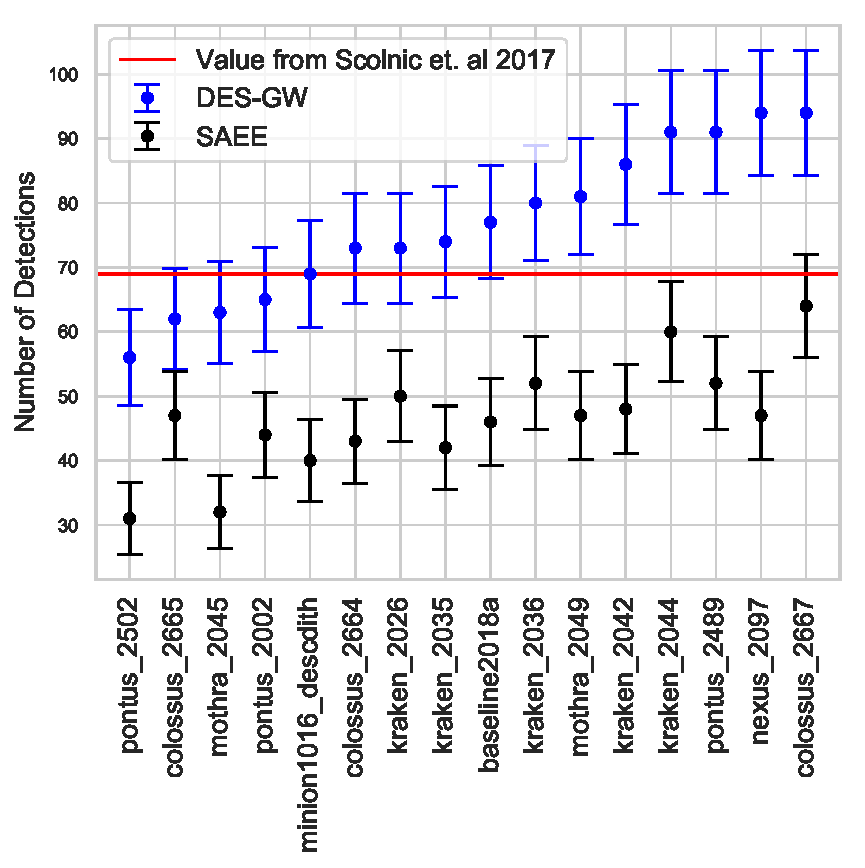
\includegraphics[scale=0.79]{figures/wfd_detection_counts_by_cadence}
  \caption{Ranking of cadence strategies for the WFD part of the survey for both KNe models, based on the number of detections found in each cadence.}
  \label{fig:cadence_ranking}
\end{figure}
\subsubsection{Results}
We rank the cadences for each KNe model based on the number of detections which pass our detections metric, see Fig. \ref{fig:cadence_ranking} and \ref{fig:cadence_ranking_ddf}. We immediately see that the DES-GW model predicts a larger number of detections than the SAEE population model. This is in part due to the early blue component, included in the DES-GW SED, being absent from the SAEE KNe model \citep{Villar2017b}. Furthermore, confirming the conclusin of \citet{Scolnic2017a}, the majority of our detections will come from the wide-fast-deep (WFD) region of the survey as opposed to the deep-drilling-fields (DDF). The typical redshift range of detected KNe, as shown in Fig. \ref{fig:typical_nz}, is between $0 \leq z \leq 0.2$, though some detections can extend out to $z \approx 0.3$. While this varies between cadences and models, this range is quite typical for all the cadences considered. The effect of changing KNe model can also be seen in Fig. \ref{fig:typical_nz}. It shows that at all redshifts the detection numbers are slightly suppressed.

\begin{figure}[h!]
  \centering
  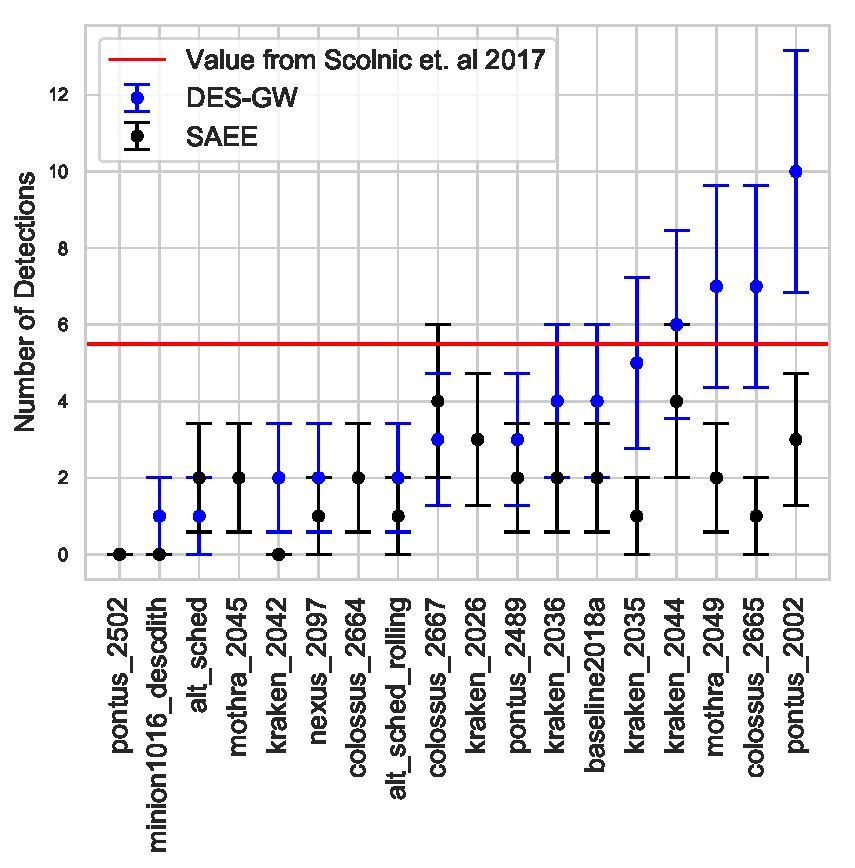
\includegraphics[scale=0.79]{figures/ddf_detection_counts_by_cadence}
  \caption{Same as the above figure, but for the DDF.}
  \label{fig:cadence_ranking_ddf}
\end{figure}

\begin{figure}[h!]
  \centering
  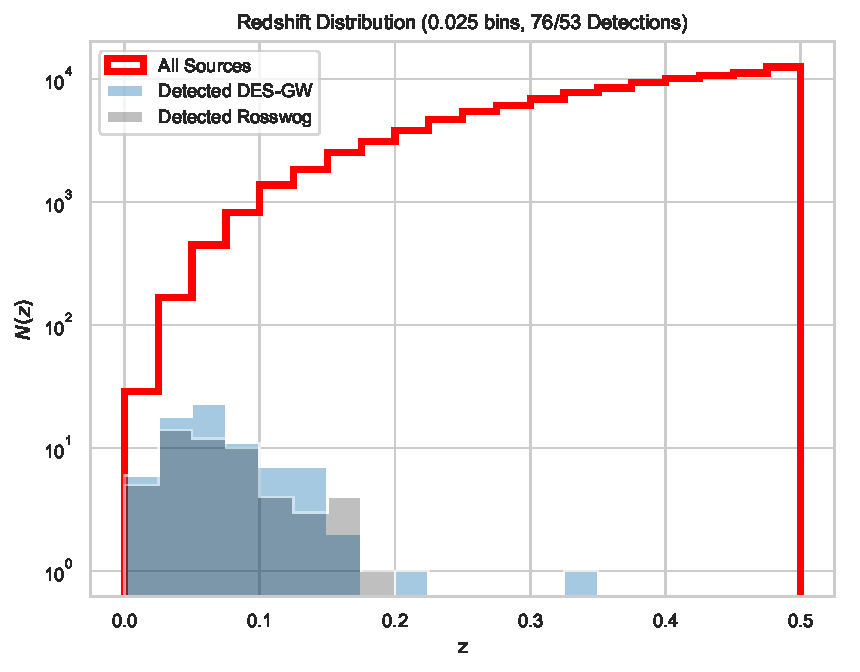
\includegraphics[scale=0.82]{figures/both_nz_base_kraken_2026}
  \caption{Example redshift distribution of detected KNe within the sample of all simulated KNe. This distribution is from the unofficial project baseline cadence \protect \textit{kraken 2026} for both the DES-GW and the SAEE KNe models. The design sensitivities of future GW detectors to detect typical binary neutron star mergers are shown by vertical lines \citep{Chen2017a, Chamberlain2017, Scolnic2017a}}
  \label{fig:typical_nz}
\end{figure}

\FloatBarrier

\newcommand{\ttt}[1]{\texttt{#1}}

\section{Large Scale Structure}
Large scale structure studies require some important features: survey uniformity over an area that maximizes the usable survey footprint with deep photometric data.  We discuss these features in the subsections below.
%%%%%%%%%%%%%%%%%%%%%%%%%%%%%%%%%%%%%%%%%%%%%%%%%%%%%%%%%%%%%%%%%%%%%%%%%%%%%%%%%%%%
\subsection{Survey Uniformity}
The effects of the LSST observing strategy on survey uniformity were explored extensively in \citet{Awan+2016}, with a follow-up in \citet[Section 9.2]{Marshall:2017wph}. The key result of these investigations is that frequent, large translational $dithers$ -- telescope-pointing offsets -- are critical to ensure survey uniformity, where $large$ is considered to be on the scale of the radius of the LSST FOV (1.75 deg). For the analyses here, we implement large, random offsets every night; note that while per-night translational dithers are not the most frequent, dithering only once per night allows for maintaining the same systematics between visit pairs and hence better calibrations. These dithers were implemented using the \ttt{MAF Stacker}, \href{https://github.com/lsst/sims_maf/blob/97988f6bc30c216fffb41e6da0a7d201e919b9ca/python/lsst/sims/maf/stackers/ditherStackers.py#L371}{RandomDitherPerNightStacker}; see more \href{https://github.com/LSSTDESC/ObsStrat/tree/issue/3/desc-dithers}{here}.

%%%%%%%%%%%%%%%%%%%%%%%%%%%%%%%%%%%%%%%%%%%%%%%%%%%%%%%%%%%%%%%%%%%%%%%%%%%%%%%%%%%%
\subsection{Optimized WFD Footprint}
Now, in order to select a galaxy sample for LSS studies, we must implement selection cuts. Specifically, to attain a Y10 gold sample at $i<25.3$, where $i$ is the $i$-band coadded 5$\sigma$ depth {\em after} accounting for MW extinction, we must require a limiting 5$\sigma$ magnitude of $i=26.0$, alongside restricting to the region with E(B-V) $<0.2$ in order to minimize the systematics induced by the uncertainties in the dust map (need a reference). Furthermore, we focus on the footprint that has coverage in all six LSST filters in order to assure good photo-$z$ quality; for Y10, this comprises $\sim$19,091 deg$^2$ in the current baseline, \ttt{baseline2018a}. Implementing our selection cuts (on coadded depth and extinction) reduces the usable footprint to $\sim$14,645 deg$^2$, hence discarding  $\sim$23\% of the WFD survey area. Figure~\ref{fig: skymaps_baseline_10yr} shows the skymaps before and after our selection cuts for the $i$-band coadded 5$\sigma$ depth after Y10.

%-------------------------------------------------------------------------------------
%-------------------------------------------------------------------------------------
\begin{figure}[H]
	\vspace*{2em}
	\centering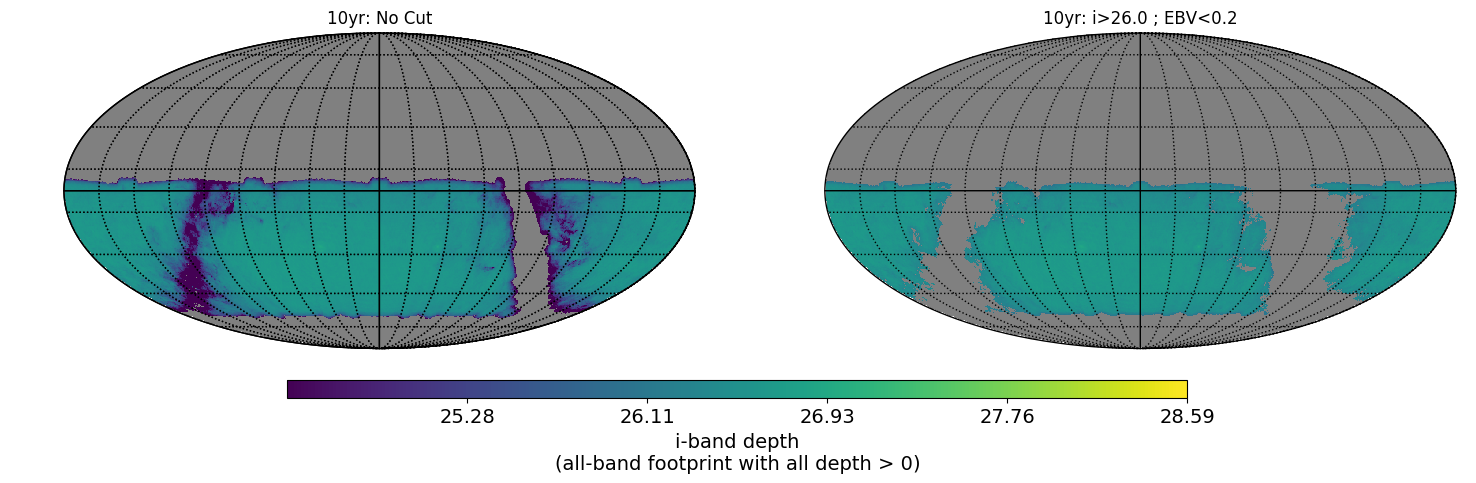
\includegraphics[width=\linewidth,trim={30 40 40 40},clip=false]{figures/lss_final_footprint_skymap_baseline2018a_nside256_RandomDitherPerNight_10yr_iband.png}
	\vspace*{1em}
	\caption{Skymaps for Y10  $i$-band coadded 5$\sigma$ depth for \ttt{baseline2018a}, limited to the footprint with coverage in all six bands, with random, per night translational dithers. \textit{Left}: Before any selection cuts.  \textit{Right}: After a depth cut of $i>26.0$ and an extinction cut of E(B-V)$<0.2$.}
	\label{fig: skymaps_baseline_10yr}
\end{figure}
%-------------------------------------------------------------------------------------

We find similar results when we implement selection cuts on Y1 data, now with a limiting 5$\sigma$ magnitude of $i=24.5$: the WFD footprint drops from $\sim$18,085 deg$^2$ to $\sim$13,613 deg$^2$, rendering $\sim$25\% of the nominal survey area unusable for our purposes.  Figure~\ref{fig: skymaps_baseline_1yr} shows the skymaps before and after our selection cuts for the $i$-band coadded 5$\sigma$  depth.

%-------------------------------------------------------------------------------------
%-------------------------------------------------------------------------------------
\begin{figure}[H]
	\vspace*{2em}
	\centering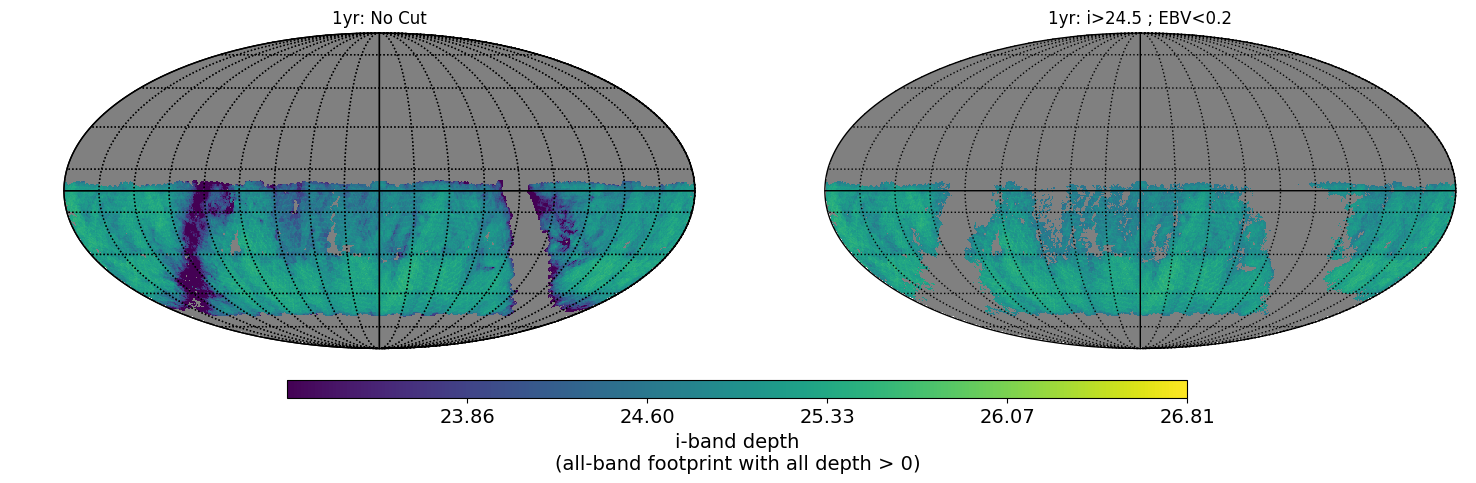
\includegraphics[width=\linewidth,trim={30 40 40 40},clip=false]{figures/lss_final_footprint_skymap_baseline2018a_nside256_RandomDitherPerNight_1yr_iband.png}
	\vspace*{1em}
	\caption{Skymaps for Y1 $i$-band coadded 5$\sigma$ depth for \ttt{baseline2018a}, limited to the footprint with coverage in all six bands with random, per night translational dithers. \textit{Left}: Before any selection cuts.  \textit{Right}: After a depth cut of $i>24.5$ and an extinction cut of $E(B-V)<0.2$.}
	\label{fig: skymaps_baseline_1yr}
\end{figure}
%-------------------------------------------------------------------------------------

In order to circumvent the issue of discarding a significant fraction of the WFD region, {\bf we propose to shift the nominal 18,000 square degree WFD footprint away from the Galactic Plane to lie {\em entirely} within the region where E(B-V)$\mathbf{<0.2}$}, allowing for optimization of the WFD footprint that is usable for our science. To illustrate this, we consider the wider-coverage \ttt{OpSim} cadence, \ttt{pontus\_2002} and implement similar selection cuts as we did for \ttt{baseline2018a}. For Y1, the final footprint consists of $\sim$15,544 deg$^2$ while Y10 footprint comprises $\sim$19,254 deg$^2$, illustrating that the WFD footprint {\em can} be optimized to yield a sufficiently large extragalactic footprint; Figures~\ref{fig: skymaps_pontus2002_10yr}-\ref{fig: skymaps_pontus2002_1yr}  show the analogs of Figures~\ref{fig: skymaps_baseline_10yr}-\ref{fig: skymaps_baseline_1yr} for \ttt{pontus\_2002}.

%-------------------------------------------------------------------------------------
%-------------------------------------------------------------------------------------
\begin{figure}[H]
	\vspace*{2em}
	\centering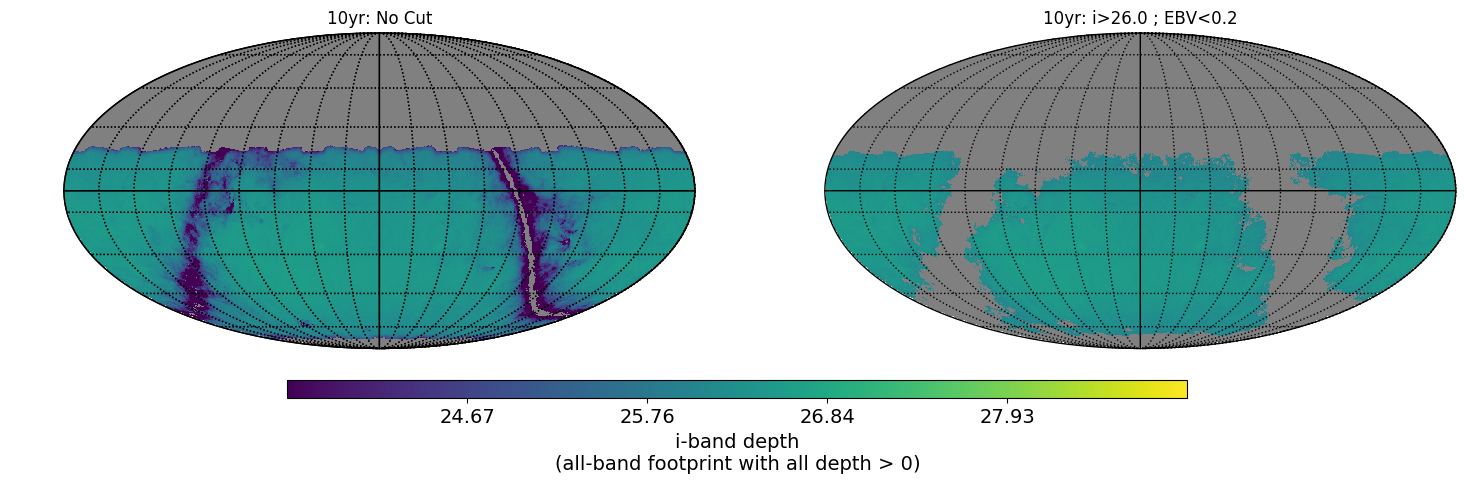
\includegraphics[width=\linewidth,trim={30 40 40 40},clip=false]{figures/lss_final_footprint_skymap_pontus_2002_nside256_RandomDitherPerNight_10yr_iband.png}
	\vspace*{1em}
	\caption{Skymaps for Y10 $i$-band coadded 5$\sigma$ depth for \ttt{pontus\_2002}, limited to the footprint with coverage in all six bands with random, per night translational dithers. \textit{Left}: Before any selection cuts.  \textit{Right}: After a depth cut of $i>26.0$ and an extinction cut of E(B-V)$<0.2$.}
	\label{fig: skymaps_pontus2002_10yr}
\end{figure}
%-------------------------------------------------------------------------------------
%-------------------------------------------------------------------------------------
%-------------------------------------------------------------------------------------
\begin{figure}[H]
	\vspace*{2em}
	\centering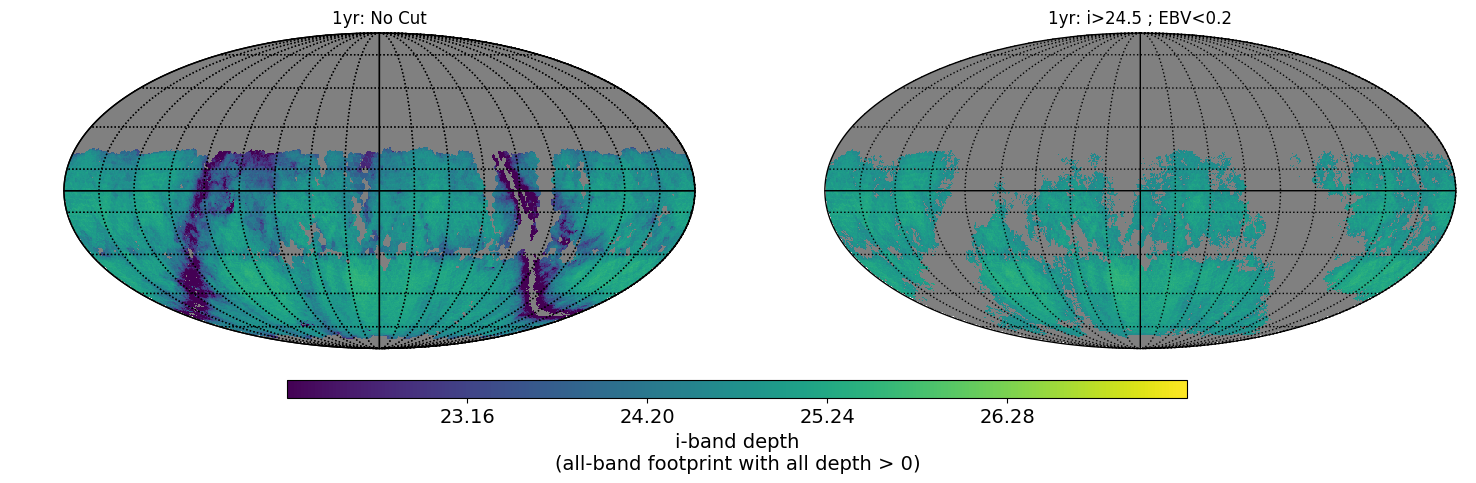
\includegraphics[width=\linewidth,trim={30 40 40 40},clip=false]{figures/lss_final_footprint_skymap_pontus_2002_nside256_RandomDitherPerNight_1yr_iband.png}
	\vspace*{1em}
	\caption{Skymaps for Y1  $i$-band coadded 5$\sigma$ depth for \ttt{pontus\_2002}, limited to the footprint with coverage in all six bands with random, per night translational dithers. \textit{Left}: Before any selection cuts.  \textit{Right}: After a depth cut of $i>24.5$ and an extinction cut of $E(B-V)<0.2$.}
	\label{fig: skymaps_pontus2002_1yr}
\end{figure}
%-------------------------------------------------------------------------------------
 Keeping these concerns in mind, we have requested a full \ttt{OpSim} run restricted to the footprint with E(B-V)$<0.2$; please see \href{https://github.com/LSSTDESC/ObsStrat/tree/issue/5/modify-wfd}{here} for more details. We are awaiting the \ttt{OpSim} output in order to assess the depth and uniformity coverage achievable in the reconfigured WFD survey area.

%%%%%%%%%%%%%%%%%%%%%%%%%%%%%%%%%%%%%%%%%%%%%%%%%%%%%%%%%%%%%%%%%%%%%%%%%%%%%%%%%%%%
\subsection{Extragalactic Footprint: Comparisons}
In order to compare the various cadences, we implement depth and extinctions cuts for four benchmarks in the ten-year survey: Y1, Y3, Y6, Y10, maintaining $i>24.5$ and $i>26.0$ cuts for Y1, Y10 respectively and extrapolating in between (hence $i>25.0$  for Y3 and $i>25.5$ for Y6). We compare the usable extragalactic footprint alongside the median $i$-band coadded 5$\sigma$ depth (to capture the achieved area and depth) and the standard deviation in the $i$-band coadded 5$\sigma$ depth (to capture the survey uniformity).

Figure~\ref{fig: compare_area} shows the footprint area for the four benchmarks for 17 different cadences. These include the baseline cadence, \ttt{baseline2018a}, the ten that are included in the WP call, and four new cadences (\ttt{kraken\_2042}, \ttt{kraken\_2044}, \ttt{mothra\_2049}, \ttt{nexus\_2097}); all these are translationally dithered post-\ttt{OpSim} simulation. We also consider five outputs from the feature-based scheduler (\ttt{cadence\_roll\_75\_mix}, \ttt{roll\_mix\_100}, \ttt{roll\_mix}, \ttt{rolling\_10yrs}, \ttt{tms\_roll\_10yrs}) and two \ttt{alt\_sched} outputs (\ttt{alt\_sched}, \ttt{alt\_sched\_rolling}); these do not need to be translationally dithered since translational dithering is built into the respective schedulers.

%-------------------------------------------------------------------------------------       
%-------------------------------------------------------------------------------------
\begin{figure}[H]
	\vspace*{2em}
	\centering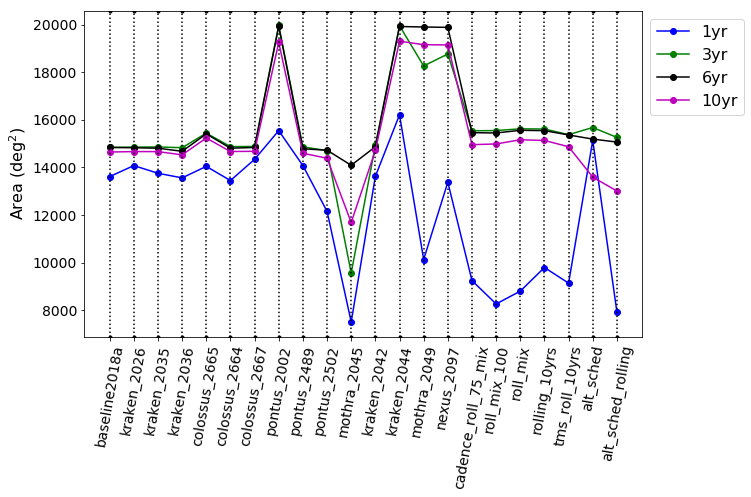
\includegraphics[width=0.5\paperwidth,trim={30 40 40 40},clip=false]{figures/lss_compare_area_22dbs.png}
	\vspace*{1em}
	\caption{Comparison of the usable survey area, following depth cuts ($i>24.5$ for Y1, $i>25.0$ for Y3, $i>25.5$ for Y6, $i>26.0$ for Y10) and an extinction cut (E(B-V)$<0.2$) for different cadences.}
	\label{fig: compare_area}
\end{figure}
%-------------------------------------------------------------------------------------

We see that for Y3, Y6, Y10, the cadences can loosely be grouped into three categories: 1) \ttt{pontus\_2002}, \ttt{kraken\_2044}, \ttt{mothra\_2049}, \ttt{nexus\_2097}, all of which yield a large usable footprint, 2) \ttt{mothra\_2045}, which performs highly unfavorably, and 3) the rest, leading to comparable final survey area.  All four cadences in the first category simulate very large WFD regions (24,700 deg$^2$); \ttt{kraken\_2044} implements single visits per night, while \ttt{mothra\_2049} and \ttt{nexus\_2097} simulate different rolling cadences. On the other hand, \ttt{mothra\_2045} implements the same rolling cadences as  \ttt{mothra\_2049} but restricts to the nominal WFD region, leading to a limited survey footprint. Based on these comparisons, we conclude that the expanded WFD footprint, even with rolling cadence, is critical for our science.  As noted above, we are proposing to shift the 18,000 deg$^2$ WFD region far enough from the Galactic plane that E(B-V)$>0.2$, which will enable greater depth to be reached than is currently realized by these expanded-footprint simulations and should allow us to fulfill the {\bf LSST SRD requirement} that the WFD offer at least 18,000 deg$^2$ over which the median number of visits is at least 825.

As for Y1, the categorization is comparatively difficult.  \ttt{pontus\_2002}, \ttt{kraken\_2044} and \ttt{alt\_sched} yield the most area while all the outputs from the feature-based scheduler and the rolling  \ttt{alt\_sched} output perform as poorly as \ttt{mothra\_2045}. One notable takeaway is that specifics of the rolling cadence are critical for Y1, as we see, e.g., that $\sim$3,000 deg$^2$ is lost between the large WFD footprint with rolling cadence in 3 declination bands vs. 2 (i.e., \ttt{nexus\_2097} vs. \ttt{mothra\_2049}).

To compare the depth and its uniformity, Figure~\ref{fig: compare_depth} shows the median (left) and the standard deviation (right) for the $i$-band coadded 5$\sigma$ depth for the 17 cadences. We observe that the cadences achieve comparable median depths, with interesting trends across the benchmarks  (e.g., \ttt{mothra\_2045} leads to deepest Y1, Y3 but shallower Y6). The uniformity is more interesting, with \ttt{mothra\_2045} significantly more non-uniform than the rest of the cadences. We note that rolling in large WFD regions leads to larger standard deviation than non-rolling, implying (again) the need to carefully select the rolling cadence specifics to be catered to the intervals planned for uniform LSST data releases.

%-------------------------------------------------------------------------------------
%-------------------------------------------------------------------------------------
\begin{figure}[H]
	\vspace*{2em}
	\begin{minipage}{.4\paperwidth}
		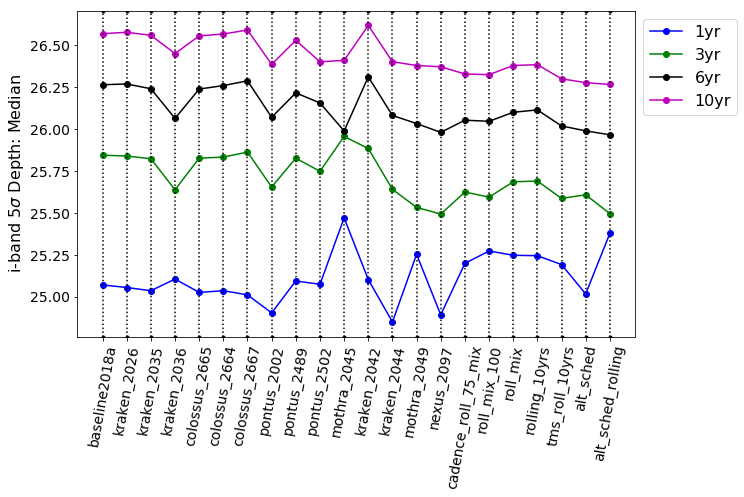
\includegraphics[width=.42\paperwidth, trim={5 20 105 10},clip=true]{figures/lss_compare_depth_median_22dbs.png}
	\end{minipage}\
	\hspace*{1em}
	\begin{minipage}{.4\paperwidth}
		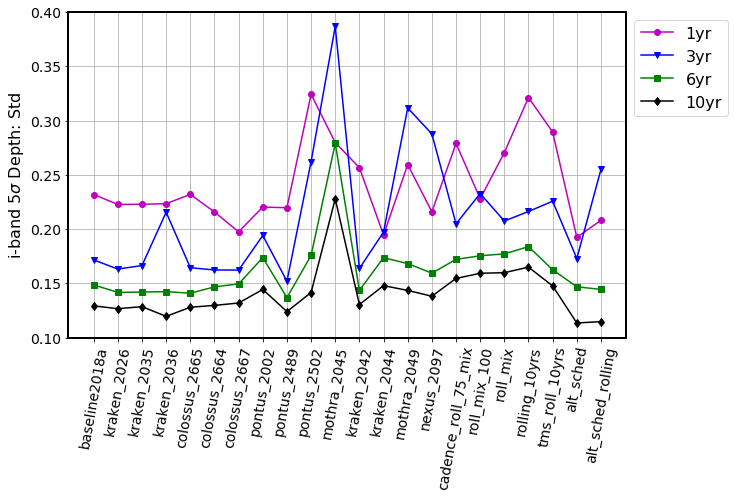
\includegraphics[width=.42\paperwidth, trim={5 20 80 10},clip=false]{figures/lss_compare_depth_std_22dbs.png}
	\end{minipage}
	\vspace*{1em}
	\caption{Comparison of two statistics on the $i$-band coadded 5$\sigma$ depth, following depth cuts ($i>24.5$ for Y1, $i>25.0$ for Y3, $i>25.5$ for Y6, $i>26.0$ for Y10) and an extinction cut (E(B-V)$<0.2$) for different cadences. \textit{Left}: Median depth. \textit{Right}: Standard deviation in the depth.}
\label{fig: compare_depth}
\end{figure}
%-------------------------------------------------------------------------------------

For exact numbers for the usable area and the depth statics, please see \href{https://github.com/LSSTDESC/ObsStrat/tree/static/static}{here}. More details about the implementation of the selection cuts are \href{https://github.com/LSSTDESC/ObsStrat/tree/static/static/depth\_cuts}{here}. 

%%%%%%%%%%%%%%%%%%%%%%%%%%%%%%%%%%%%%%%%%%%%%%%%%%%%%%%%%%%%%%%%%%%%%%%%%%%%%%%%%%%%
\subsection{To Dos for LSS}
\begin{enumerate}
\item Currently working on confirming that the OS systematics discussed in \citet{Awan+2016} are subdominant. Should be done in a few days.
\item Waiting on the \ttt{OpSim} output for the optimized WFD footprint to see how the depth improves once we have restricted to the optimized WFD footprint and check this against the 825 median visit requirement.
\item Update seeing model to utilize Eric N.'s clear 0.18'' amplitude seasonal seeing variation and consider a tapered edge to WFD to cover a wider dec range in good seeing and a smaller one in bad.  This is necessary for final optimization of the 18,000 deg$^2$ WFD region.
\item Translational dithering currently leads to shallower survey edges, given that the dithered pointings sometimes lead to partial coverage outside the nominal footprint. A solution to this issue is an "annealed" dither pattern, which preferentially rejects dithers outside the defined survey region.
%*** This might not be something to worry about if the feature-based scheduler is adopted as the official scheduler as there would be no need to dither post-\ttt{Opsim} simulation.  
%***EG:  Actually, we should ask Peter Yoachim if FBS does annealing, otherwise this will be just as big of a problem with it.  He may not have thought about this yet, and it's actually easier for us to handle with a post-processing dither than for him to handle with precessed tilings and *no* dithers!  
\end{enumerate}

%%%%%%%%%%%%%%%%%%%%%%%%%%%%%%%%%%%%%%%%%%%%%%%%%%%%%%%%%%%%%%%%%%%%%%%%%%%%%%%%%%%%
\subsection{To Dos: Miscellaneous - May Belong In Other Sections}
\begin{enumerate}
\item Optimize distribution of time spent in each filter for photometric redshift quality.  Melissa has runs going for this, with a clear initial indication that more $u$-band is justified for $z>1.2$ but only small variations seen at $z<1.2$ (except for radically dumb changes).
\item Need to explore a clever rotational dither strategy that enables more frequent rotational dithers while ensuring that visit pairs are conducted at the same \ttt{rotSkyPos} angle. Or we can show that using a single randomly chosen value of \ttt{rotTelPos} each night is feasible as the sky rotates and that this approach yields a sufficiently uniform distribution of \ttt{rotTelPos} and \ttt{rotSkyPos} values over the ten-year survey.
\item Propagate through to cosmology, using scaling relations that Tim is developing.  First need to implement scaling from Chang+13 to propagate galaxy detection depth through to Neff for weak lensing.  But David K. points out that WL is also dependent upon S/N for ellipticity measurements; need to iron out how that can be estimated from \ttt{OpSim} and fed into Tim's forecasts.
  
\end{enumerate}

 

\section{Photometric Redshifts}\label{sec:pz}

A one page summary of our analysis of the {\tt OpSim} and {\tt ALTSched} results is provided in Section \ref{mlg_sec:pz_summary}. A more in-depth evaluation of how the photometric redshifts derived from LSST photometry will evolve over the 10 year survey, for a variety of observing strategies that includes the formal {\tt OpSim} runs along with more general scenarios in which e.g., 5\% of the total observing time is redistributed to or from each filter in turn, is currently underway and being documented in this Overleaf draft: \url{https://www.overleaf.com/read/fgnvddbnrmgk}.


% % % % % % % % % % % % % % % % % % % % % % % % % % % % %
\subsection{Evaluating the Photometric Evolution of the Observing Strategies}\label{ssec:pz_opsim_phot}

To evaluate the photometric quality produced by each of the proposed observing strategies, we use the Metric Analysis Framework (MAF) as follows.

{\bf Slicer:} We use a HEALpix slicer with {\tt nside} $=16$ and a random dither to the field RA and Dec ({\tt latCol = randomDitherFieldPerNightRa} and {\tt lonCol = randomDitherFieldPerNightDec}). This slicer returns metrics in fields with an approximate resolution of $220$ arcminutes ($3.67$ degrees), similar to a single LSST pointing, and the dither helps to smooth out field-to-field variations in a realistic way. The dither option is not needed or applied with simulations from the feature-based scheduler ({\tt rolling\_10yrs}) or {\tt ALTSched}. 

{\bf Metric:} We use {\tt ExgalM5}, which returns the $5{\sigma}$ limiting magnitude for a given filter, corrected for Galactic dust extinction. We require that a given field have observations in all $6$ filters to be considered as conceivably be appropriate for photo-$z$ estimation (and recall that we impose the constraint that a galaxy must be {\it detected} in $griz$ to get a photo-$z$ estimate). We furthermore impose that the Galactic extinction $E(B-V) \leq 0.2$ mag and that the $5{\sigma}$ $i$-band detection limit be at least $24.5/25.0/25.5/26.0$ magnitudes at $1/3/6/10$ years.

{\bf Bundle:} We run the metric and slicer for years $1$, $3$, $6$, and $10$. We only consider images that are obtained as part of the WFD survey component, to avoid depth pockets from mini-surveys or deep drilling fields. We furthermore only consider fields with a Galactic longitude of $60 < l < 300$ degrees {\em or} Galactic latitude of $b>30$ degrees, as would a cosmological science analysis relying on the LSST photo-$z$, but the $E(B-V) \leq 0.2$ mag is actually more constraining than this location constraint.

Using the above slicer, metric, and bundle, we generate a single file per year per {\tt OpSim} or {\tt ALTSched} run, in which each row represents a ``field" that was observed in all $6$ filters as part of the WFD survey, and the columns are right ascension, declination, and the $5{\sigma}$ limiting magnitude in filters $ugrizy$. It turns out that many of the {\tt OpSim} runs result in a similar evolution for the median limiting magnitude for each filter as a function of survey year, and thus would not produce different photo-$z$ results, except for these three: {\tt pontus\_2002}, which has a larger WFD survey area of $24700$ square degrees ($-78 < \delta < +18$); {\tt pontus\_2489}, which does $20$-second visits in $grizy$ filters and $40$-second visits in $u$-band, increasing the $u$-band depth and leading to a larger total number of visits in the others filters; and {\tt rolling_10yrs}, a rolling cadence that alternates between two bands of declination. 


% % % % % % % % % % % % % % % % % % % % % % % % % % % % %
\subsection{The CMNN Photo-$z$ Estimator}\label{ssec:pz_exp_cmnn}

For this work we have used the color-matched nearest-neighbors (CMNN) photometric redshift estimator from \cite[][herafter G18]{2018AJ....155....1G}. The CMNN should not be taken as representing the ``best" photo-$z$ estimator or the ``official" LSST algorithm -- it is neither of these things. It is a simple algorithm that produces photo-$z$ results of a statistical quality that directly correlates with the photometric quality of the input, and thus is very useful for evaluating the impact on photo-$z$ of any changes to the LSST photometric quality -- such as the {\tt OpSim} runs that we consider in this work.

As described in G18, this estimator uses a training set of galaxies with known redshifts and a test set for which photo-$z$ are to be estimated. For each galaxy in the test set, the estimator first identifies a color-matched subset of training galaxies by calculating the Mahalanobis distance in color-space between the test galaxy and all training-set galaxies. The Mahalanobis distance in this case is the difference between the test- and training-set galaxy color, divided by the photometric error of the test-set galaxy color, summed over all available colors (Equation 1 in G18). Then, a threshold value is applied that defines a ``good" color match. This threshold is set by the percent point function (PPF): for example, for $N_{\rm dof}=5$, PPF$=95$ per cent of all training galaxies consistent with the test galaxy will have $D_M < 11.07$ (where $N_{\rm dof}$, the number of degrees of freedom, is the number of colors). The estimator then chooses one of the color-matched training-set galaxies (e.g. the nearest-neighbor or a random selection), and uses that galaxy's known redshift as the test-set galaxy's photo-$z$ (a "redshift donor"). The uncertainty in the photo-$z$ estimate is taken to be the standard deviation of the true redshifts of training-set galaxies in the color-matched subset. 

Compared to G18, there are some minor differences in how this photo-$z$ estimator was applied in this work. Here, we require that a test-set galaxy be detected in the LSST filters $griz$ and thus have colors $g-r$, $r-i$, and $i-z$ or else a photo-$z$ estimate is not attempted, and we've used a threshold of PPF=$0.68$ to define the color-matched subset of training galaxies. Unlike G18, we choose randomly from the color-matched subset of training galaxies instead of choosing the nearest neighbor. This difference leads to less accurate and less precise photometric redshifts, but by using a random selection in the photo-$z$ estimator, the {\tt OpSims} runs that degrade/enhance the LSST photometry end up having a larger relative impact on the resulting photometric redshifts. This helps with the experiment at hand, which is to assess the relative impacts of different {\tt OpSim} runs, and {\em not} to generate the best possible photo-$z$ results for each {\tt OpSim} run.

As a final note, to accelerate processing time, we have applied both the color and magnitude pre-cuts to the training set, as described in G18. The color cut is fairly benign, but the magnitude pre-cut effectively works as a ``pseudo-prior" by cutting down the training set to the 10\% of training galaxies with an $i$-band magnitude nearest to the test galaxy's $i$-band magnitude. The ``pseudo-prior" may improve accuracy of the photo-$z$ estimate for some, but can also introduce a bias in the results. Since all of the experiments in this work will be looking at {\it relative} changes to the photo-$z$ quality as various inputs are changed, this kind of degradation to the {\it absolute} photo-$z$ quality is acceptable in this case.


% % % % % % % % % % % % % % % % % % % % % % % % % % % % %
\subsection{Simulating LSST Photometry for the Training and Test Catalogs} \label{ssec:pz_exp_cats}

For this work we use the same simulated mock galaxy catalog as used in G18. This catalog contains the ``true" redshift and the ``true" apparent magnitudes in $ugrizy$ for all galaxies. The training and test set galaxies are drawn randomly from this catalog. We use $1\times10^6$ galaxies for the training set, and $5\times10^4$ galaxies for the test set. Justification for the sizes of the test and training sets is provided in G18, but here we note that the size of the test set is adequate to achieve statistical measures in the high-$z$ bins.

For the training set, we simulate observed apparent magnitudes for all galaxies assuming that the $5{\sigma}$ photometric depths in each filter are equivalent to the LSST baseline 10-year survey: $u=26.09,g=27.38,r=27.53,i=26.83,z=26.06,y=24.86$. This is the same as what was used in G18. For the test set, we also simulate observed apparent magnitudes for all galaxies using the $5{\sigma}$ photometric depths in each filter, but these depths change for the different LSST observing strategies that we consider in this work. We randomly assign each test galaxy to one of the simulated ``fields" from our MAF, as described above in Section \ref{ssec:pz_opsim_phot}. For all training- and test-set galaxies, once we know the $5{\sigma}$ photometric depth to apply, we derive the expected photometric error based on each galaxy's ``true" catalog magnitude (using Equation 5 from \citealt{2008arXiv0805.2366I}), and then add a random scatter proportional to this uncertainty to simulate observational uncertainties. This method is described in more depth, with plots of error {\it vs.} apparent magnitude, in G18.

In all of our experiments, both the test and training sets are limiting to $i<25$ mag, so that we are simulating photo-$z$ for samples of ``good" galaxies. Furthermore, in our implementation of the CMNN algorithm, galaxies are required to have at least 3 colors or else a photo-$z$ estimate is not attempted. Thus, our results represent the photo-$z$ quality of a ``gold'' sample of galaxies for cosmological analyses, and do not reflect any impact on the survey area or number of galaxies available for a cosmological analyses -- only the photo-$z$ quality of the ``best'' observed galaxies.


% % % % % % % % % % % % % % % % % % % % % % % % % % % % %
\subsection{Analysis Methodology}\label{ssec:pz_exp_meth}

We take these blurbs from G18 to describe our statistical measures of photo-$z$ quality and the common plot styles that we will use to represent our results. For this analysis we will use only the point estimates of photo-$z$ for each of our test galaxies, although CMNN is capable of returning a full posterior (e.g., Schmidt et al. 2018, in prep.). Although we have included simulated galaxies with $z<0.3$ and $z>3$ in both the test and training sets, our analysis focuses on a cosmological set of galaxies with $0.3 \leq z_{\rm phot} \leq 3$.

{\bf Statistical Measures --} Where $z_{\rm true}$ is the ``true" catalog redshift and $z_{\rm phot}$ is the photo-$z$, the error is $\Delta z_{(1+z)} = (z_{\rm true} - z_{\rm phot})/(1+z_{\rm phot})$. Including a factor of $(1+z)$ in the denominator acts to compensate for larger uncertainties at high-$z$. For all of our results we calculate the robust standard deviation in $\Delta z_{(1+z)}$ as the FWHM of the interquartile range (IQR) divided by $1.349$ ($\sigma_{\rm IQR}$) and the robust bias as the mean value of $\Delta z_{(1+z)}$ in the IQR ($\overline{\Delta z_{\rm(1+z), IQR}}$). We reject catastrophic outliers ($|z_{\rm spec}-z_{\rm phot}| > 1.5$) from the IQR before calculating the standard deviation and bias, {\em which is different from our analyses in past work} such as \cite{2018AJ....155....1G}. We bootstrap our uncertainties on these statistical measures by randomly drawing a subsets and recalculating the statistics 1000 times. Outlier galaxies are identified as those with $\Delta z_{(1+z)} > 3\sigma_{\rm IQR}$ or $\Delta z_{(1+z)} > 0.06$, whichever is {\it larger}, where $\sigma_{\rm IQR}$ is calculated from all galaxies in $0.3 \leq z_{\rm phot} \leq 3.0$ (i.e., outliers are defined globally). The fraction of outlier galaxies that we calculate {\it includes} catastrophic outliers (as defined above).

{\bf Plot Styles --} To visualize our photo-$z$ results we create plots that compare the true $vs.$ photometric redshifts, in which outlier galaxies are typically colored red and a solid line of $z_{\rm true} = z_{\rm phot}$ is drawn to guide the eye. These plots are useful to obtain a global sense of the photo-$z$ quality and the structure in the outliers positions, especially the features that are perpendicular to the $z_{\rm true} = z_{\rm phot}$, which represent photo-$z$ degeneracies caused by the Balmer break passing between filters. We also plot the robust standard deviation, robust bias, and fraction of outliers as a function of $z_{\rm phot}$, typically as a way to directly compare the bulk photo-$z$ results of experiments in which the simulated galaxy photometry has been altered in some way. 


% % % % % % % % % % % % % % % % % % % % % % % % % % % % %
\subsection{Results}\label{ssec:pz_results}

As discussed in Section \ref{ssec:pz_opsim_phot}, only three of the {\tt OpSim} runs result in a significantly different evolution in the median photometric depth of WFD fields compared to the baseline, and so we only simulate photo-$z$ results for the following: 

\begin{itemize}
\item {\tt OpSim} {\tt kraken\_2026}, the baseline run
\item {\tt OpSim} {\tt pontus\_2002}, a larger WFD survey area of $24700$ square degrees ($-78 < \delta < +18$)
\item {\tt OpSim} {\tt pontus\_2489}, $20$-second visits in $grizy$ filters and $40$-second visits in $u$-band, increasing the $u$-band depth and leading to a larger total number of visits in the others filters
\item {\tt OpSim} {\tt rolling_10yrs}, a rolling cadence that alternates between two bands of declination
\item {\tt ALTSched} {\tt altched\_baseline}, the baseline run
\item {\tt ALTSched} {\tt altsched\_rolling}, a rolling cadence that alternates between two bands of declination
\end{itemize}

In Figure \ref{fig:tzpz} we plot the true {\it vs.} the photometric redshifts at years $1$, $3$, and $10$ of the LSST survey, for each of the four {\tt OpSim} runs considered in this work. While the improvement over the years of the survey is easily noticed in these plots (compare columns), very little distinction is visible in the photo-$z$ results for the different {\tt OpSim} runs (compare rows). For this reason, we do not include the {\tt ALTSched} results in this format. The following plots of statistical measures are more useful in this regard.

In Figure \ref{fig:stats_opsim} we compare the statistical measures of robust standard deviation and bias from the IQR (after the rejection of catastrophic outliers), and the fraction of outliers (including catastrophic) as a function of photo-$z$ bin for each of the four considered {\tt OpSim} runs, at $1$ and $10$ years of the LSST survey. We draw the following conclusions from Figure \ref{fig:stats_opsim}. 
\begin{itemize}
\item Extending the survey area to $-78 < \delta < +18$ for a large WFD area of $24,700$ square degrees (green line; {\tt pontus\_2002}) results in degraded photo-$z$ quality compared to the baseline (blue line; {\tt kraken\_2026}). This degradation is most clearly seen in redshift bins $1.5 \lesssim z_{\rm phot} \lesssim 2.2$ at 1 year.
\item The 20/40s "many visits" option that lengthens the $u$-band exposure time to $40$ seconds and shortens it to $20$ seconds in $grizy$ (orange line; {\tt pontus\_2489}) performs similarly to the baseline, but with a small but significant improvement in the standard deviation and fraction of outliers at $z_{\rm phot} \gtrsim 1.5$.
\item The rolling cadence that alternates between two declination bands ({\tt rolling\_10yrs}; magenta line) produces degraded results that are similar to those from extending the total WFD area (green line).
\end{itemize}

In Figure \ref{fig:stats_altsched} we compare the statistical measures of robust standard deviation and bias from the IQR (after the rejection of catastrophic outliers), and the fraction of outliers (including catastrophic) as a function of photo-$z$ bin for the {\tt OpSim} baseline and rolling cadence to the {\tt ALTSched} baseline and rolling cadence. We draw the following conclusions from Figure \ref{fig:stats_altsched}. 
\begin{itemize}
\item The {\tt OpSim} and {\tt ALTSched} baselines deliver equivalent results in terms of photo-$z$ quality.
\item The {\tt ALTSched} rolling cadence delivers the better photo-$z$ at year 1 across all redshift bins than the {\tt OpSim} rolling cadence, or either simulator's baseline. We attribute this to the fact that {\tt ALTSched}'s rolling cadence does not spend any time observing the deprioritized declination band, whereas {\tt OpSim}'s {\tt rolling\_10yrs} allows it $25\%$ of the baseline number of visits.
\item Of these four simulations, the {\tt OpSim} baseline cadence delivers the best photo-$z$ at year 10.
\end{itemize}

In Figure \ref{fig:evol} we chart the evolution in the statistical measures over year of the survey in redshift bins of $0.8 \leq z_{\rm phot} \leq 1.2$  and $1.8 \leq z_{\rm phot} \leq 2.2$. We can see that all four {\tt OpSim} runs progress in a similar fashion {\it except} for the rolling cadence with two declination bands done in alternating years (magenta line; {\tt rolling\_10yrs}), which shows a mild improvement at year 1 (but recall the improved statisics would only apply to half of the sky area). The {\tt ALTSched} rolling cadence shows an even more pronounced improvement at year 1, but by year 10 is consistent with the baseline cadence.

In Table \ref{tab:zbins} we provide the relative robust standard deviation results in two redshift bins, $0.3<z_{\rm phot}<1.5$ and $1.5<z_{\rm phot}<3.0$, for years 1, 3, 6, and 10, for each of the considered {\tt OpSim} and {\tt ALTSched} runs. Note that these redshift bins are not the same as those used for Figure \ref{fig:evol}. These results are reported as {\it relative to} the baseline robust standard deviation for the low-$z_{\rm phot}$ bin at LSST year 10 (i.e., all values of the robust standard deviation are divided by this value). Note that the ``many visits" survey ({\tt pontus\_2489}) {\it performs better than the {\tt OpSim} baseline in the high-$z$ bin for all years}, and has an equivalent performance to the baseline in the low-$z$ bin.

\begin{figure}
\begin{center}
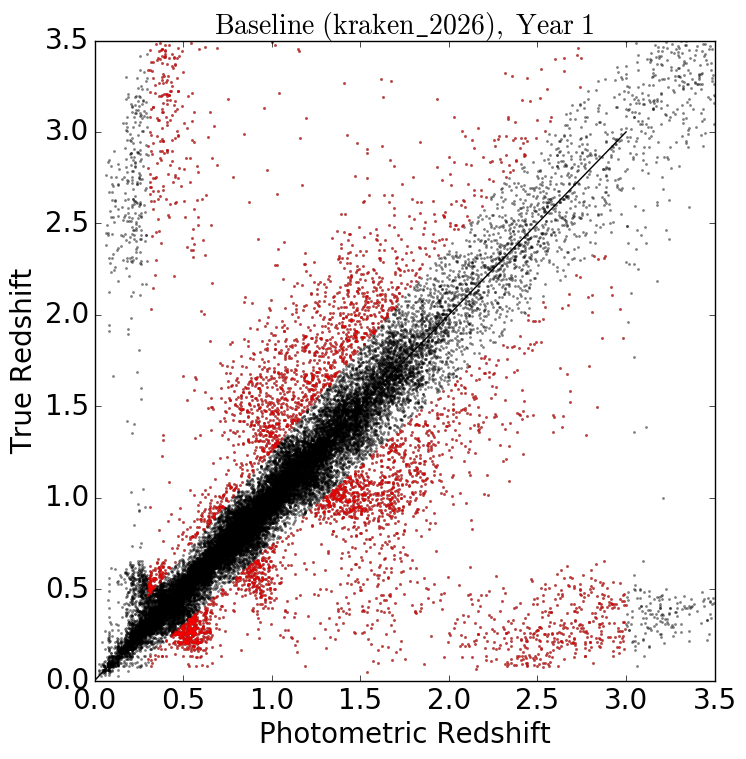
\includegraphics[width=5cm,trim={0cm 0cm 0cm 0cm},clip]{figures/tzpz_kraken2026_1.png}
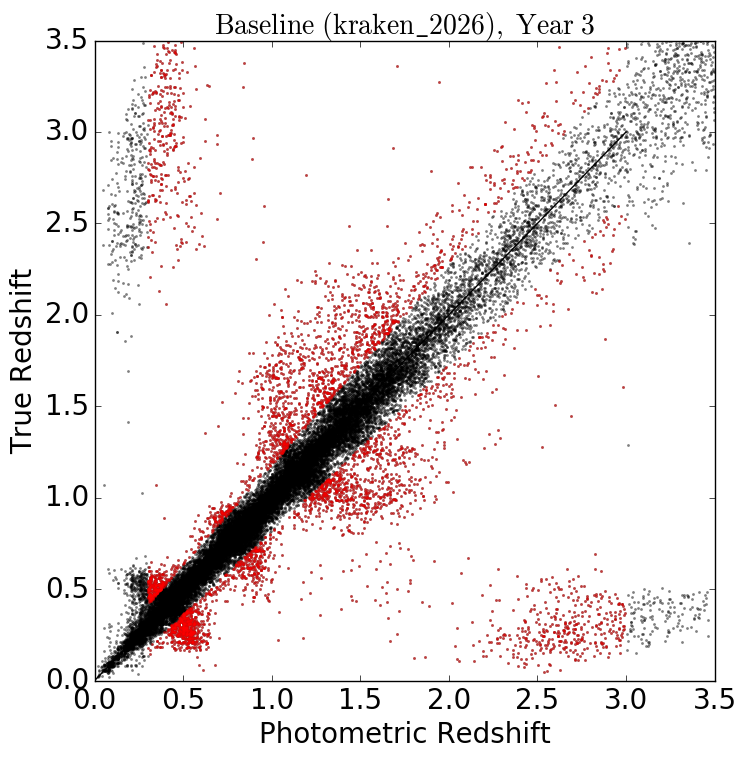
\includegraphics[width=5cm,trim={0cm 0cm 0cm 0cm},clip]{figures/tzpz_kraken2026_3.png}
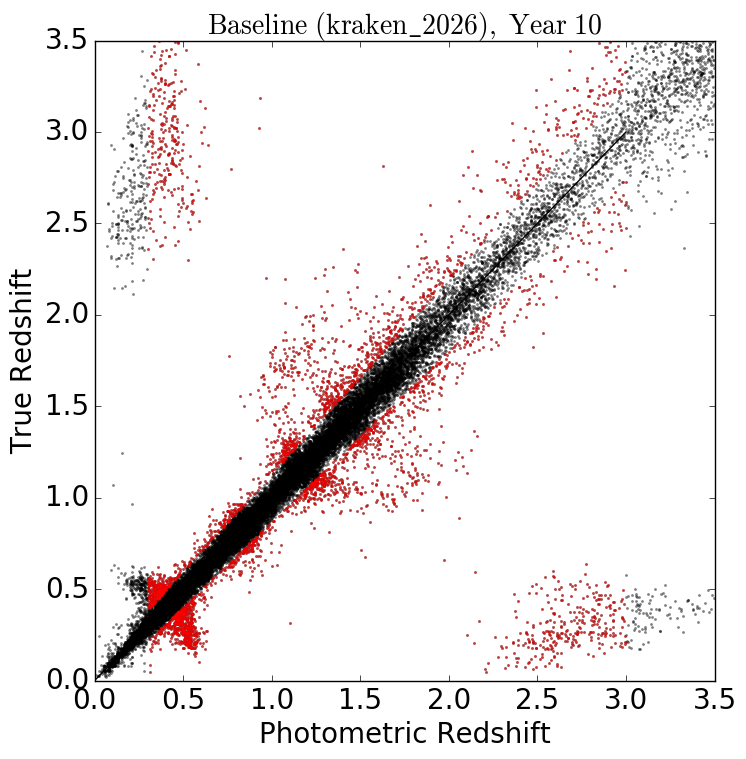
\includegraphics[width=5cm,trim={0cm 0cm 0cm 0cm},clip]{figures/tzpz_kraken2026_10.png}
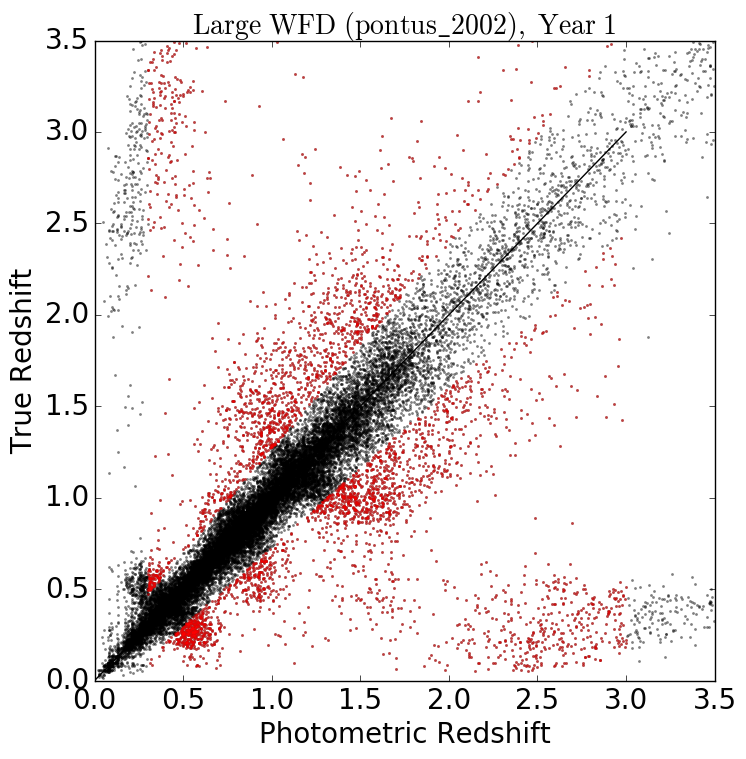
\includegraphics[width=5cm,trim={0cm 0cm 0cm 0cm},clip]{figures/tzpz_pontus2002_1.png}
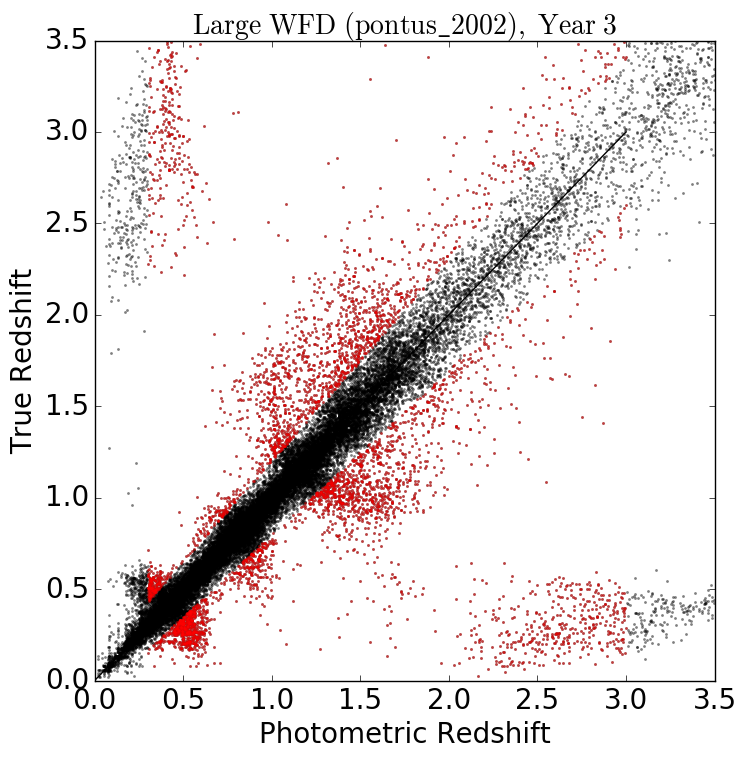
\includegraphics[width=5cm,trim={0cm 0cm 0cm 0cm},clip]{figures/tzpz_pontus2002_3.png}
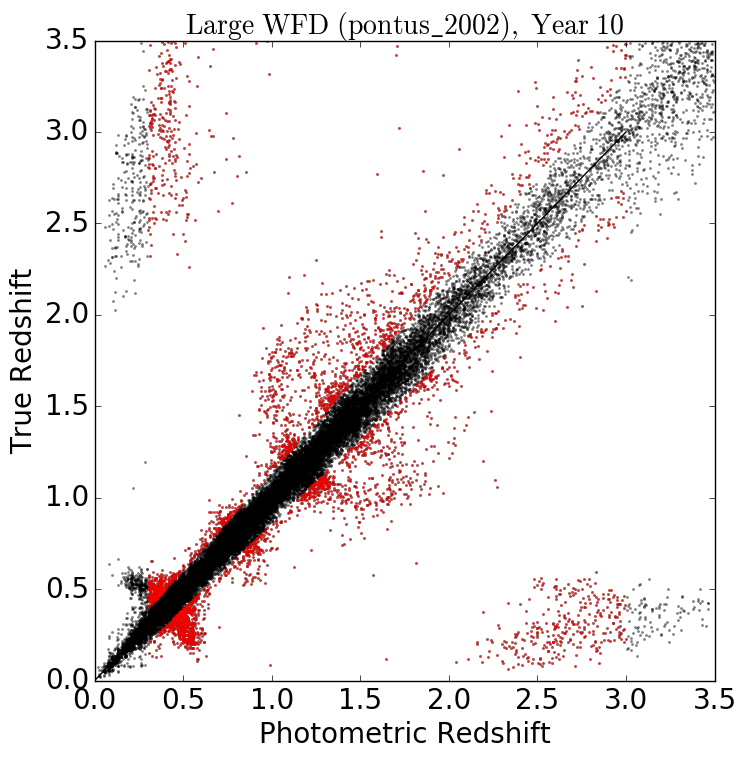
\includegraphics[width=5cm,trim={0cm 0cm 0cm 0cm},clip]{figures/tzpz_pontus2002_10.png}
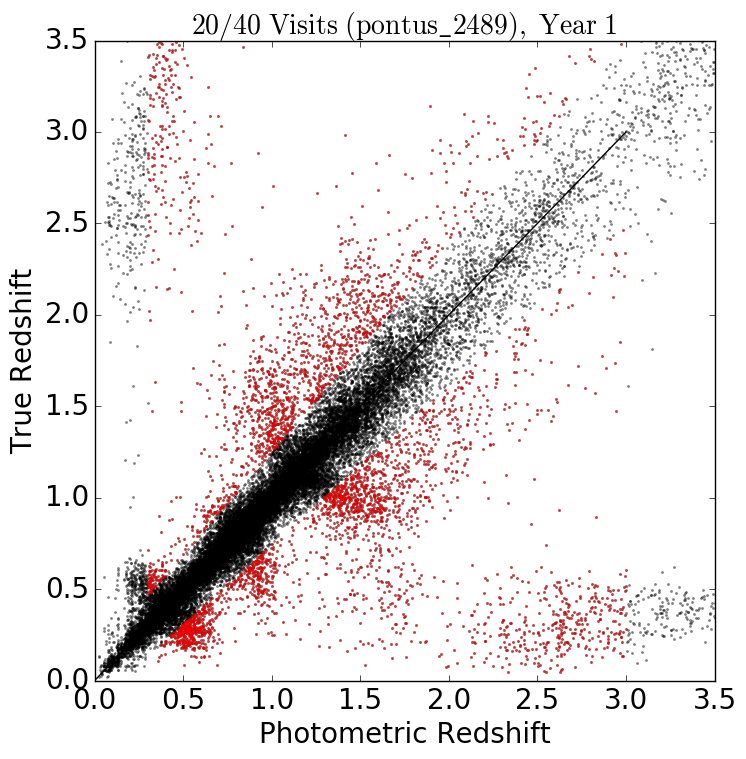
\includegraphics[width=5cm,trim={0cm 0cm 0cm 0cm},clip]{figures/tzpz_pontus2489_1.png}
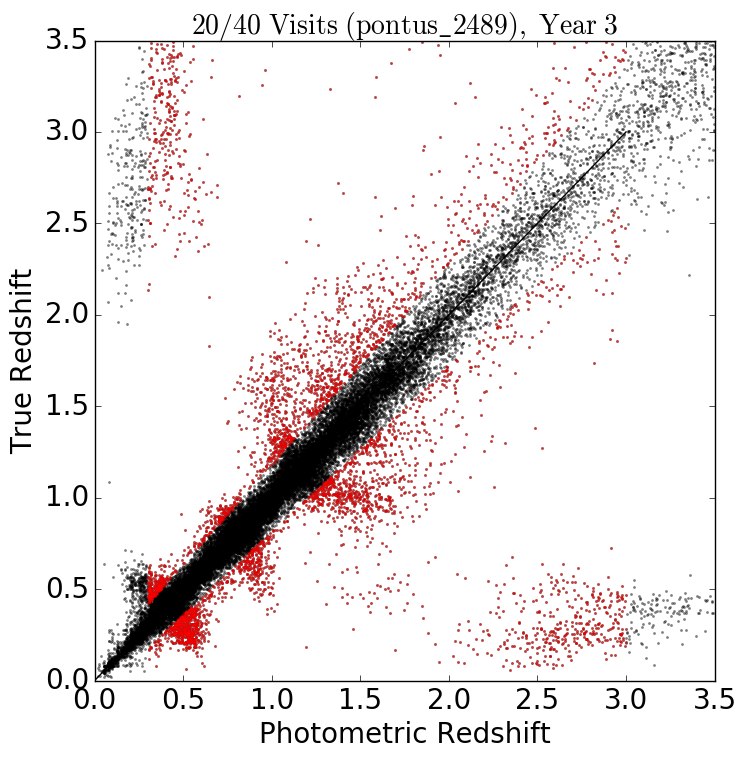
\includegraphics[width=5cm,trim={0cm 0cm 0cm 0cm},clip]{figures/tzpz_pontus2489_3.png}
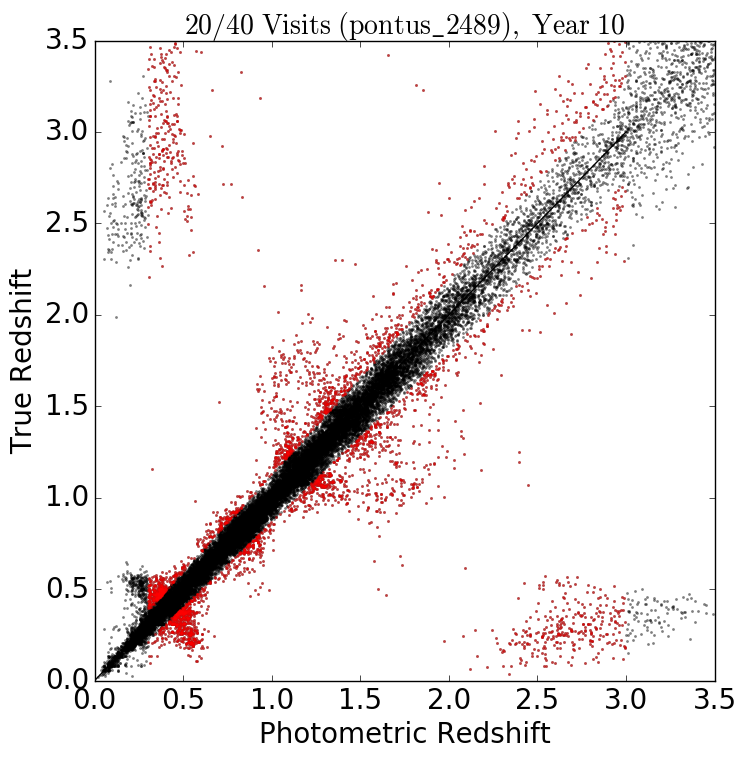
\includegraphics[width=5cm,trim={0cm 0cm 0cm 0cm},clip]{figures/tzpz_pontus2489_10.png}
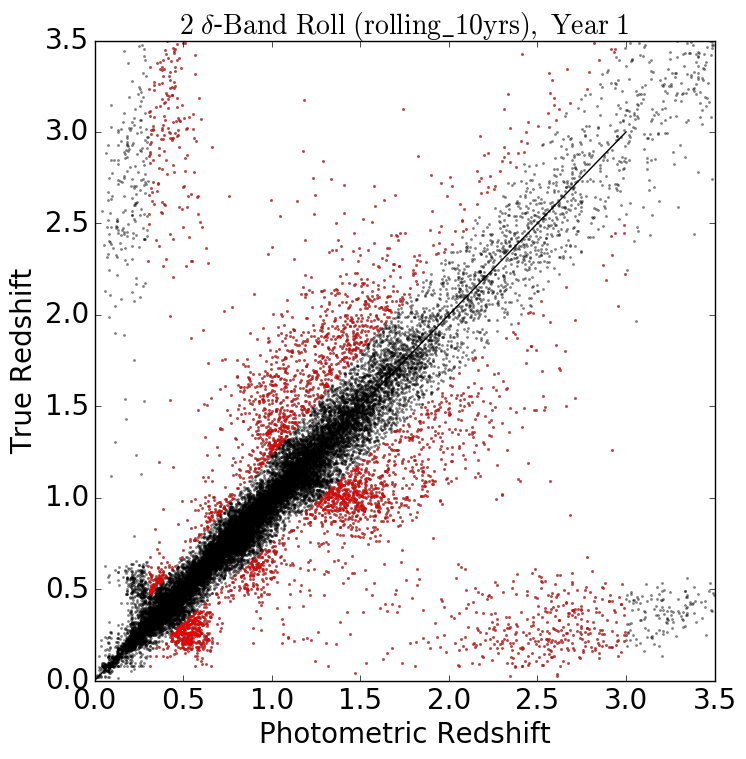
\includegraphics[width=5cm,trim={0cm 0cm 0cm 0cm},clip]{figures/tzpz_rolling10yrs_1.png}
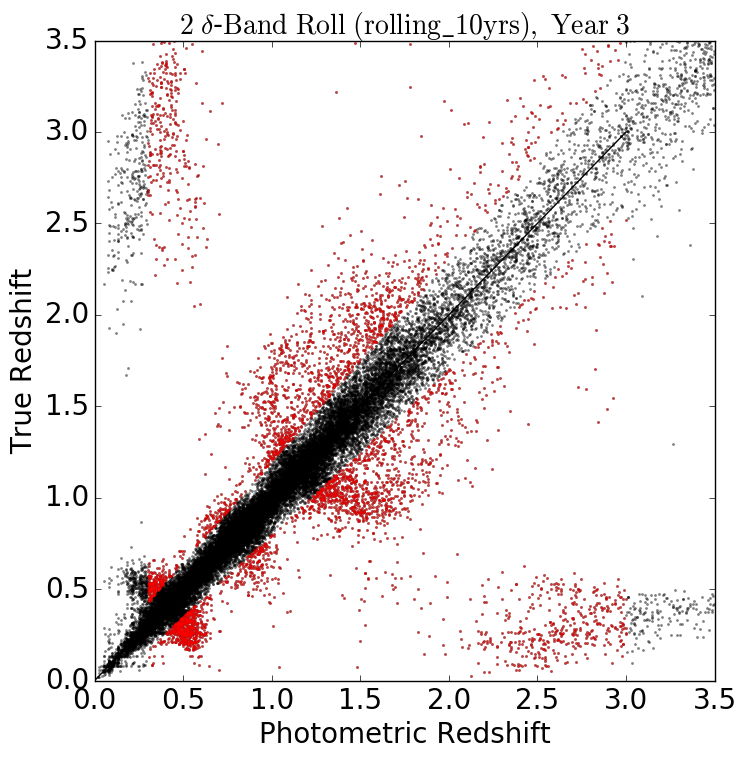
\includegraphics[width=5cm,trim={0cm 0cm 0cm 0cm},clip]{figures/tzpz_rolling10yrs_3.png}
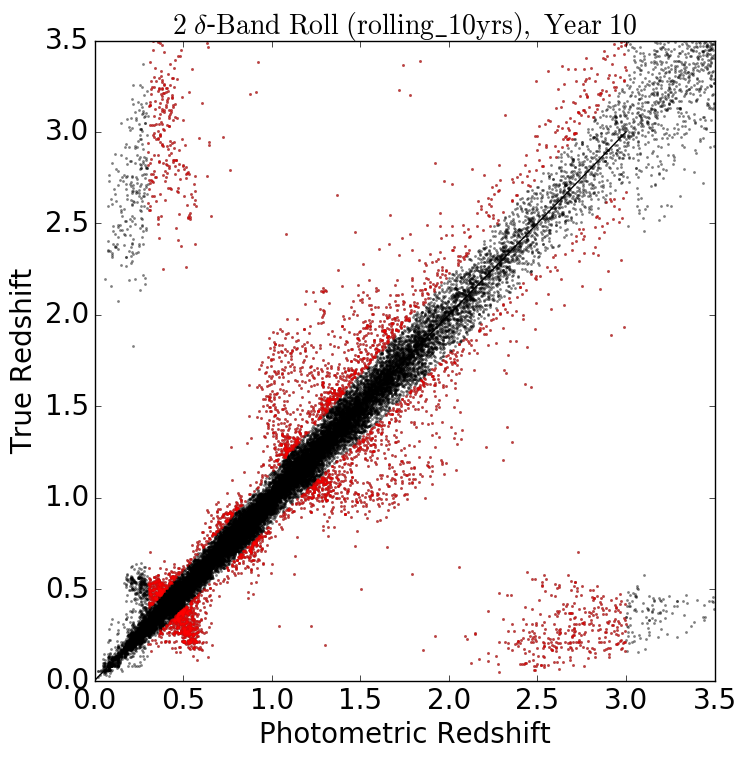
\includegraphics[width=5cm,trim={0cm 0cm 0cm 0cm},clip]{figures/tzpz_rolling10yrs_10.png}
\caption{True {\it vs.} photometric redshifts for all test galaxies, with statistical outliers plotted as red points. Columns from left to right represent results at years 1, 3, and 10. Rows from top to bottom represent results from the {\tt OpSim} baseline ({\tt kraken\_2026}), large WFD area with declinations including  $-78<\delta<+18$ degrees ({\tt pontus\_2002}), the ``many visits" strategy with 40/20 second exposures in $u$/$grizy$ filters ({\tt pontus\_2489}), and a rolling cadence with two declination bands ({\tt rolling\_10yrs}). Results from {\tt ALTSched} are not plotted in this way. \label{fig:tzpz}}
\end{center}
\end{figure}

\begin{figure}
\begin{center}
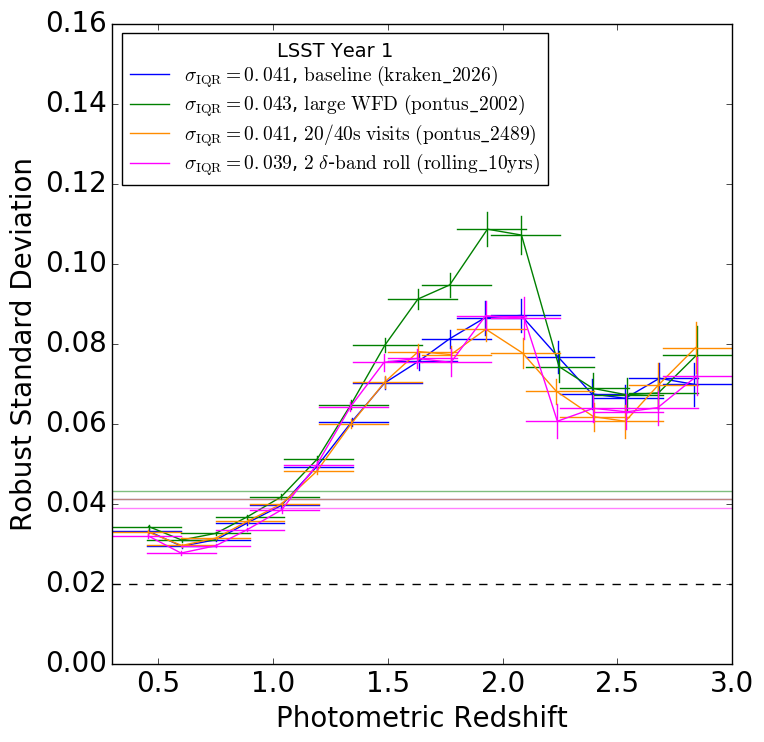
\includegraphics[width=7cm,trim={0cm 0cm 0cm 0cm},clip]{figures/year1_IQRs.png}
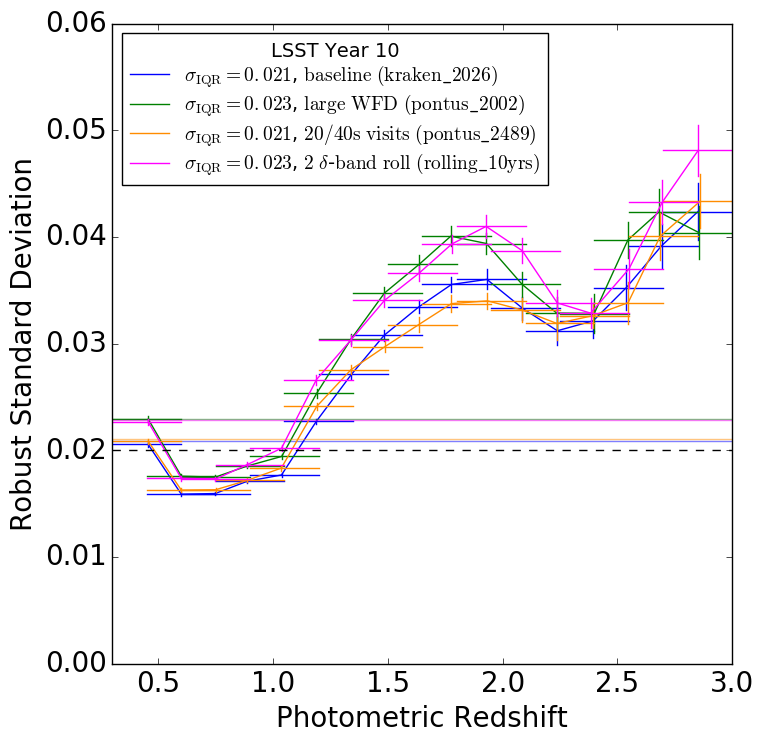
\includegraphics[width=7cm,trim={0cm 0cm 0cm 0cm},clip]{figures/year10_IQRs.png}
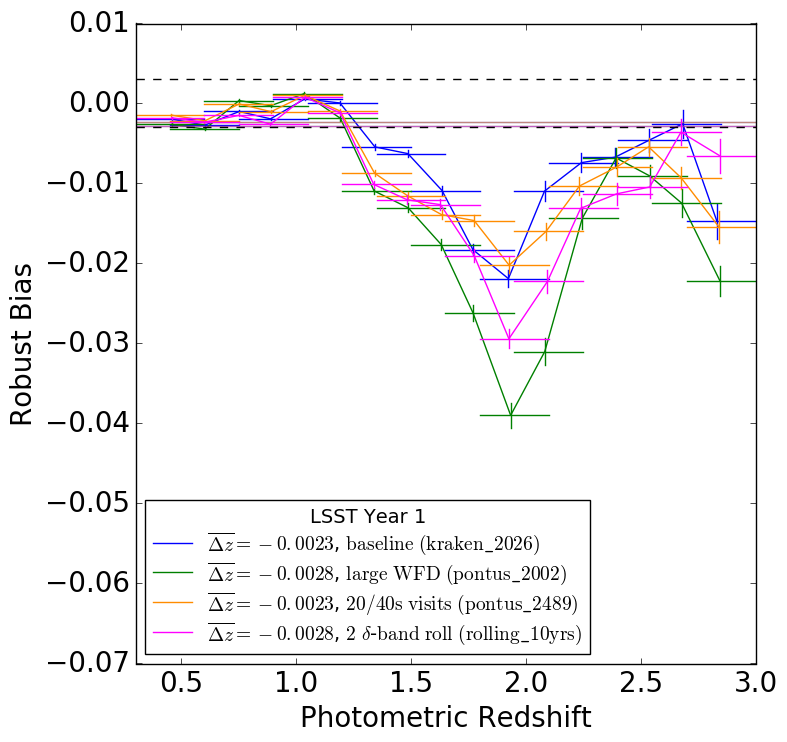
\includegraphics[width=7cm,trim={0cm 0cm 0cm 0cm},clip]{figures/year1_bias.png}
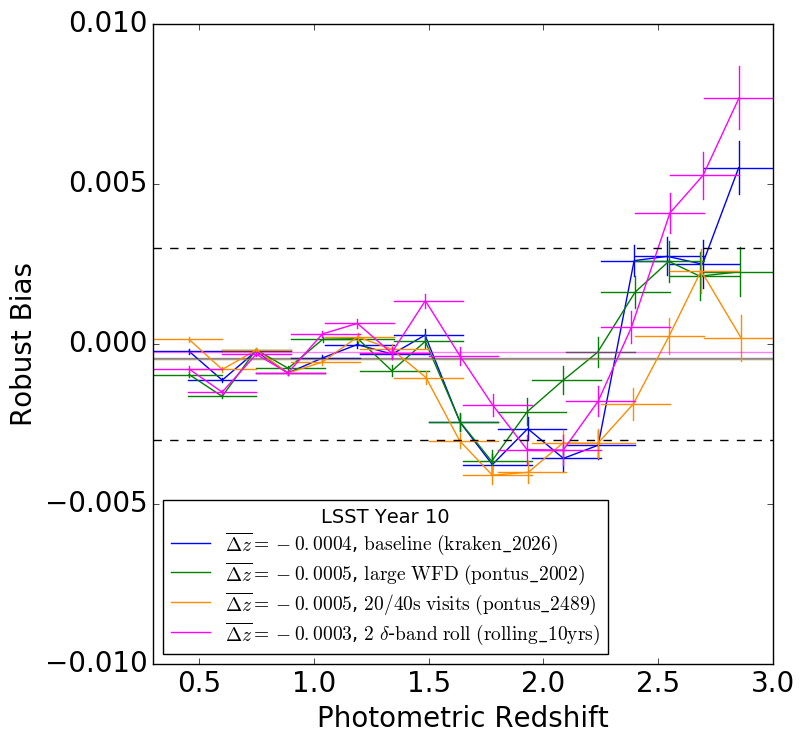
\includegraphics[width=7cm,trim={0cm 0cm 0cm 0cm},clip]{figures/year10_bias.png}
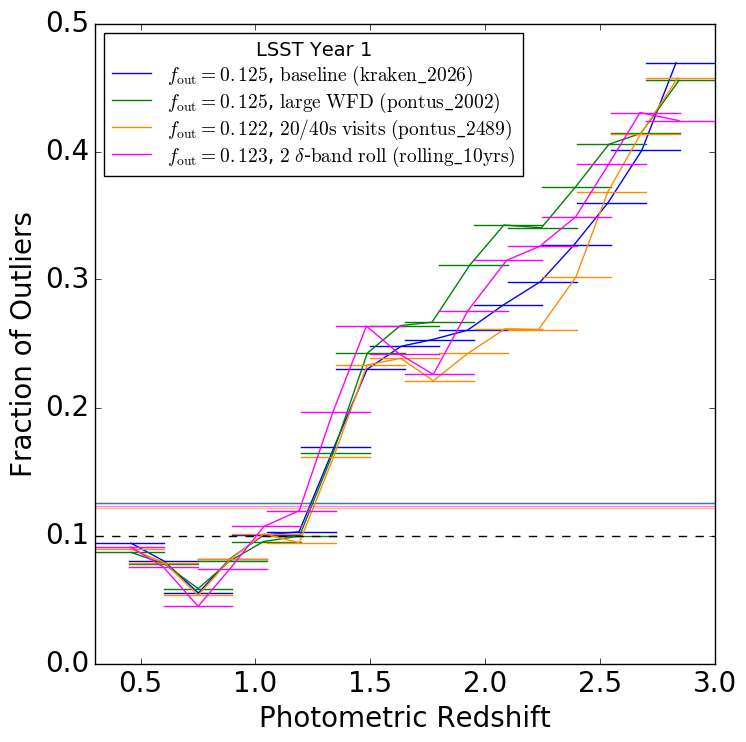
\includegraphics[width=7cm,trim={0cm 0cm 0cm 0cm},clip]{figures/year1_fout.png}
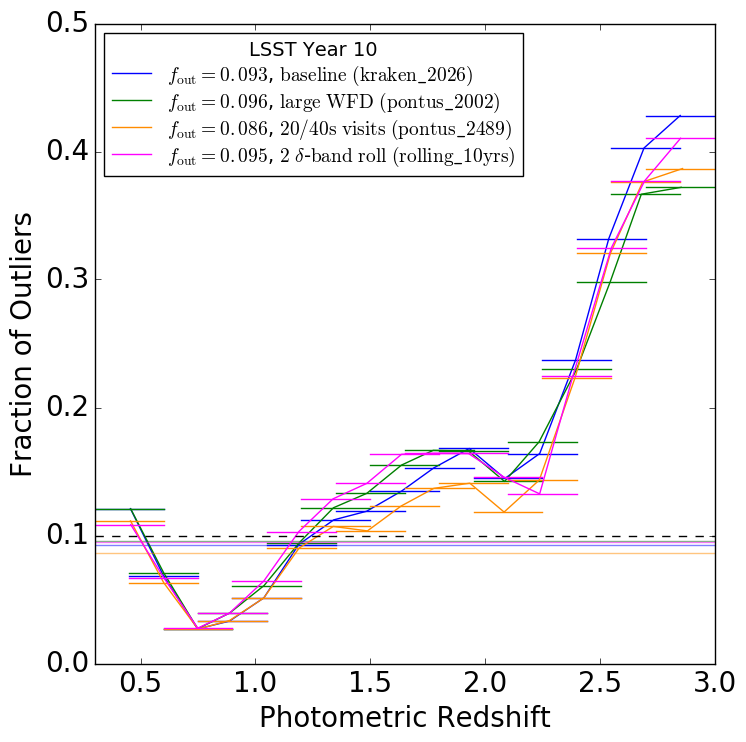
\includegraphics[width=7cm,trim={0cm 0cm 0cm 0cm},clip]{figures/year10_fout.png}
\caption{Statistical measures of robust standard deviation (from the IQR; top), robust bias (middle), and fraction of outliers (bottom) as a function of photo-$z$, at years $1$ (left column) and $10$ (right column). Note that the $y$-axes are not matched between columns. Results are presented for the baseline ({\tt kraken\_2026}; blue), large WFD area with declinations including  $-78<\delta<+18$ degrees ({\tt pontus\_2002}; green), the ``many visits" strategy with 40/20 second exposures in $u$/$grizy$ filters ({\tt pontus\_2489}; orange), and a rolling cadence with two declination bands ({\tt rolling\_10yrs}; magenta). Horizontal dashed line represents the LSST Science Requirement Document's target for a photo-$z$ bin of $0.3 \leq z_{\rm phot} \leq 3.0$., and horizontal colored bars represent the statistical for a photo-$z$ bin of $0.3 \leq z_{\rm phot} \leq 3.0$. \label{fig:stats_opsim}}
\end{center}
\end{figure}

\begin{figure}
\begin{center}
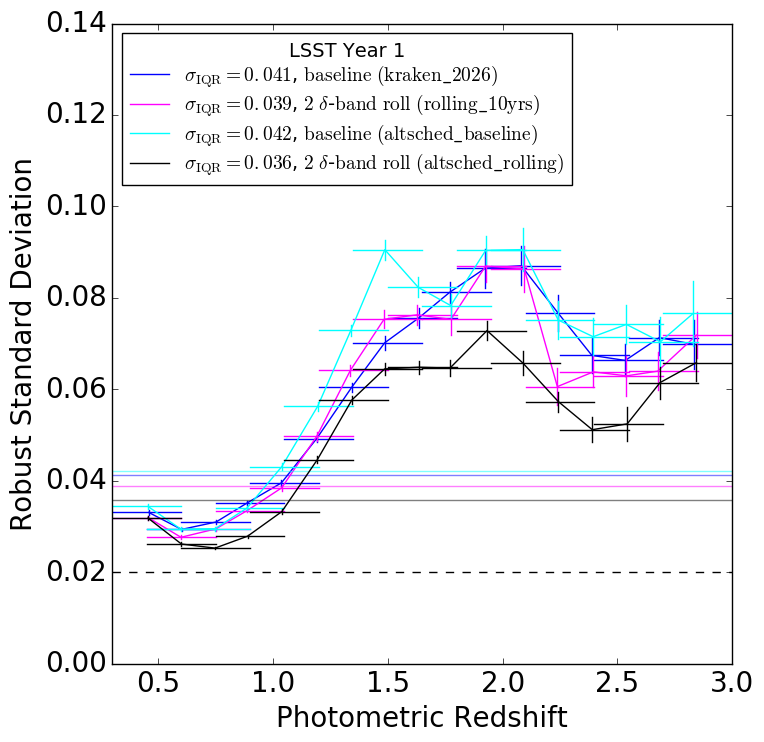
\includegraphics[width=7cm,trim={0cm 0cm 0cm 0cm},clip]{figures/ALTyear1_IQRs.png}
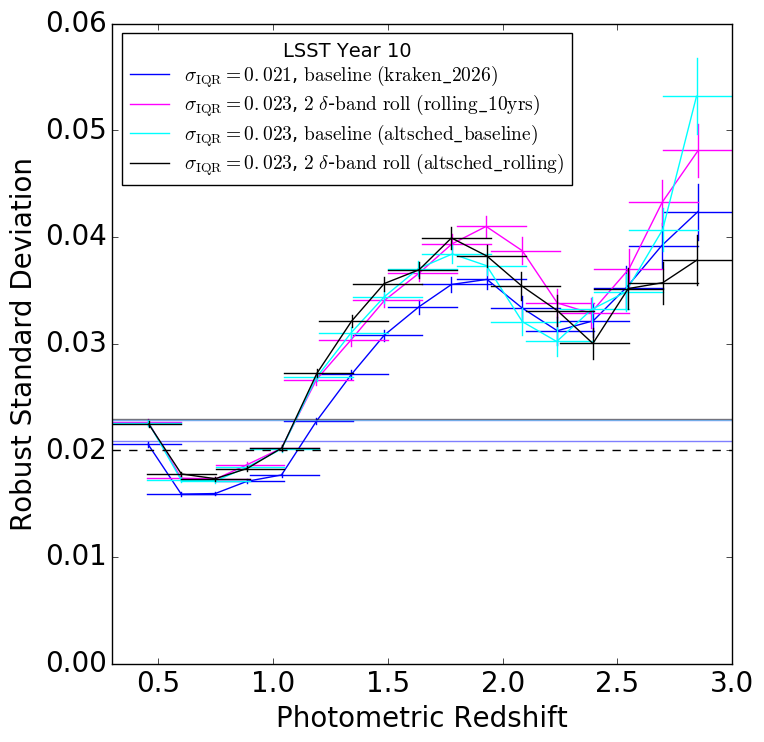
\includegraphics[width=7cm,trim={0cm 0cm 0cm 0cm},clip]{figures/ALTyear10_IQRs.png}
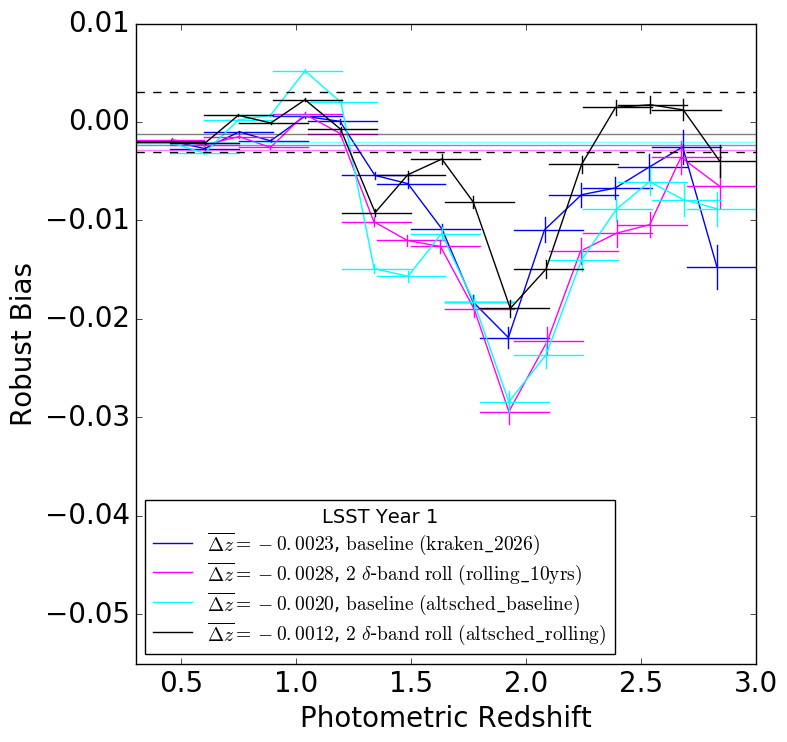
\includegraphics[width=7cm,trim={0cm 0cm 0cm 0cm},clip]{figures/ALTyear1_bias.png}
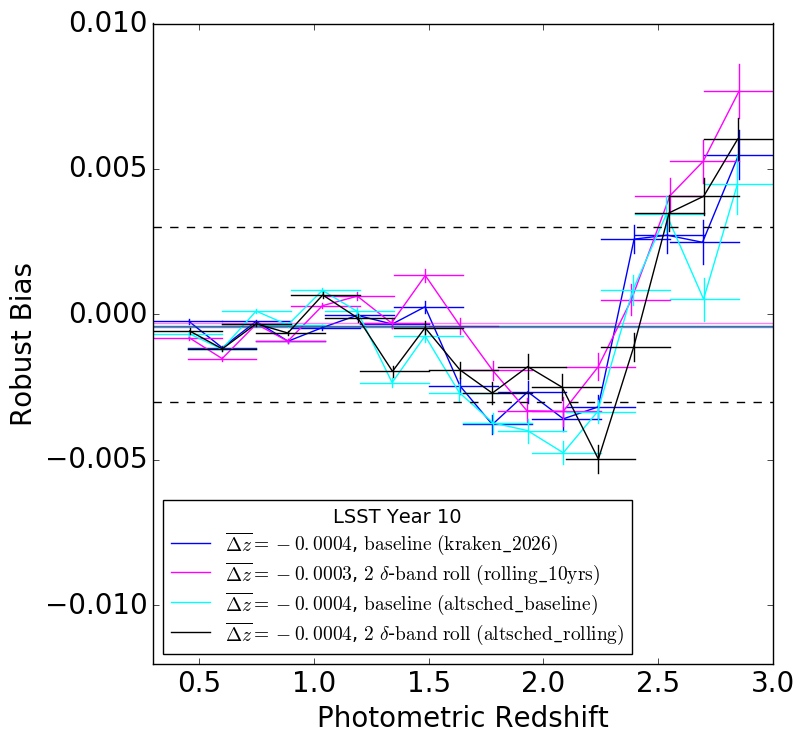
\includegraphics[width=7cm,trim={0cm 0cm 0cm 0cm},clip]{figures/ALTyear10_bias.png}
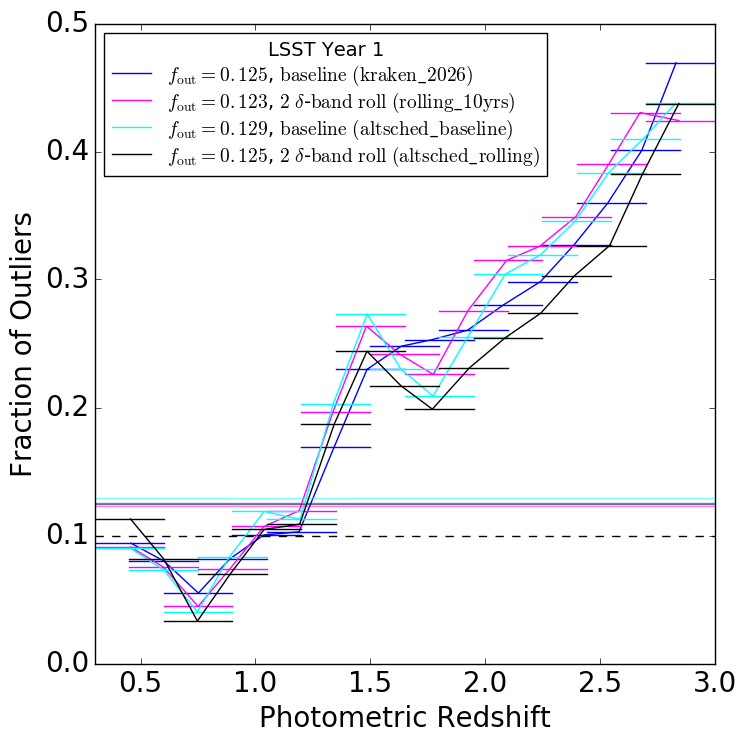
\includegraphics[width=7cm,trim={0cm 0cm 0cm 0cm},clip]{figures/ALTyear1_fout.png}
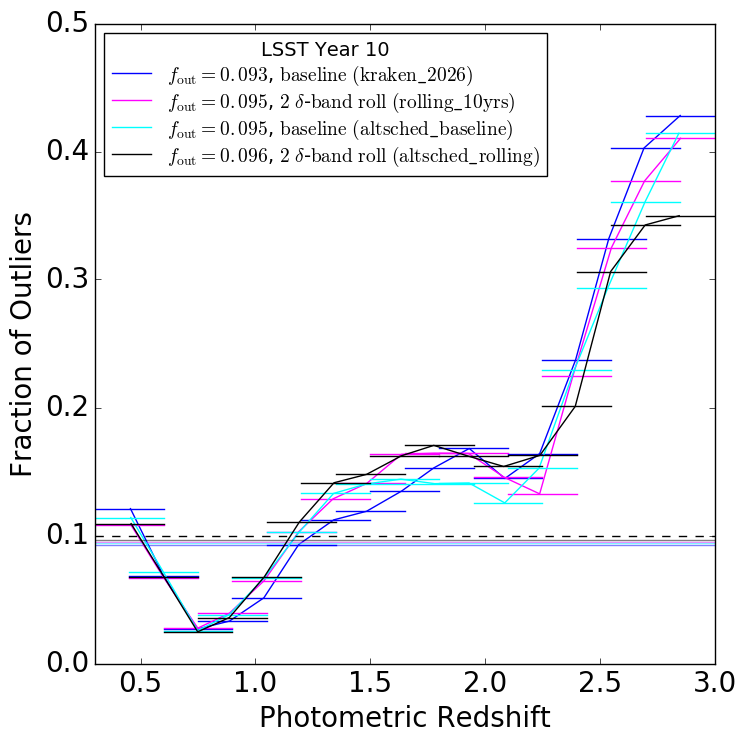
\includegraphics[width=7cm,trim={0cm 0cm 0cm 0cm},clip]{figures/ALTyear10_fout.png}
\caption{Statistical measures of robust standard deviation (from the IQR; top), robust bias (middle), and fraction of outliers (bottom) as a function of photo-$z$, at years $1$ (left column) and $10$ (right column). Note that the $y$-axes are not matched between columns. Results are presented for the {\tt OpSim} baseline ({\tt kraken\_2026}; blue) and rolling cadence ({\tt rolling\_10yrs}; magenta), and the {\tt ALTSched} baseline ({\tt altsched\_baseline}; cyan) and rolling cadence ({\tt altsched\_rolling}; black). Horizontal dashed line represents the LSST Science Requirement Document's target for a photo-$z$ bin of $0.3 \leq z_{\rm phot} \leq 3.0$., and horizontal colored bars represent the statistical for a photo-$z$ bin of $0.3 \leq z_{\rm phot} \leq 3.0$. \label{fig:stats_altsched}}
\end{center}
\end{figure}

\begin{figure}
\begin{center}
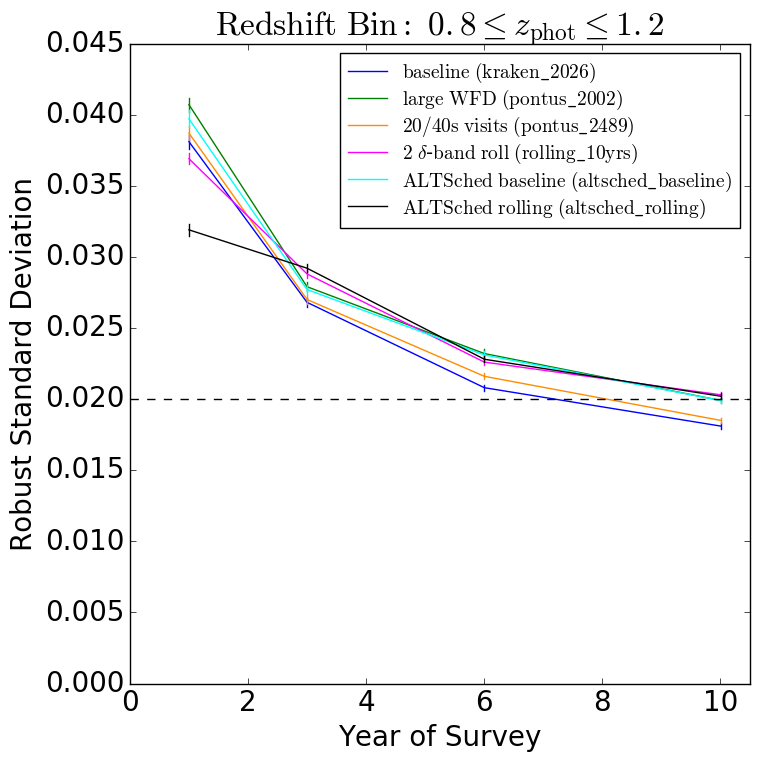
\includegraphics[width=7cm,trim={0cm 0cm 0cm 0cm},clip]{figures/zbin1_IQRs.png}
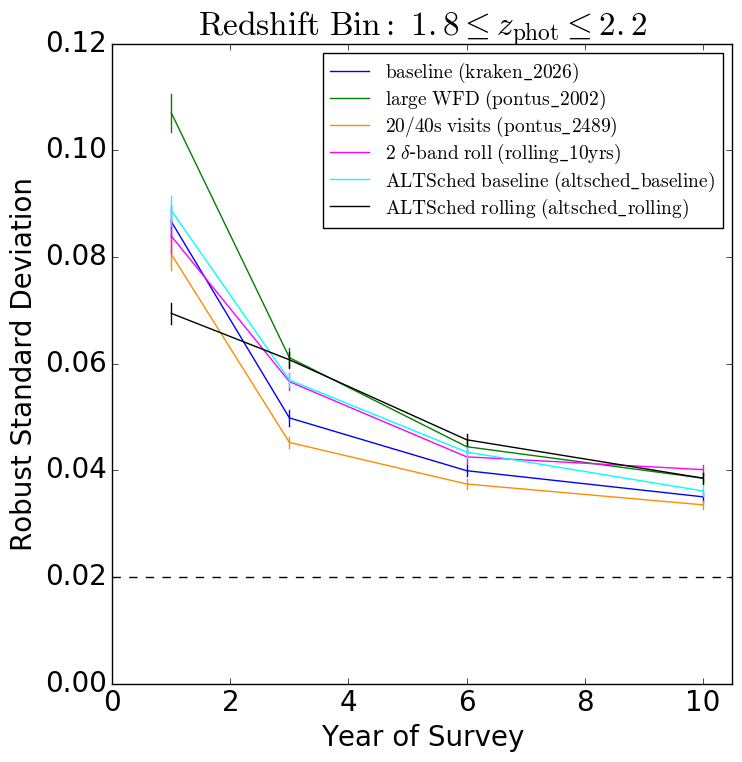
\includegraphics[width=7cm,trim={0cm 0cm 0cm 0cm},clip]{figures/zbin2_IQRs.png}
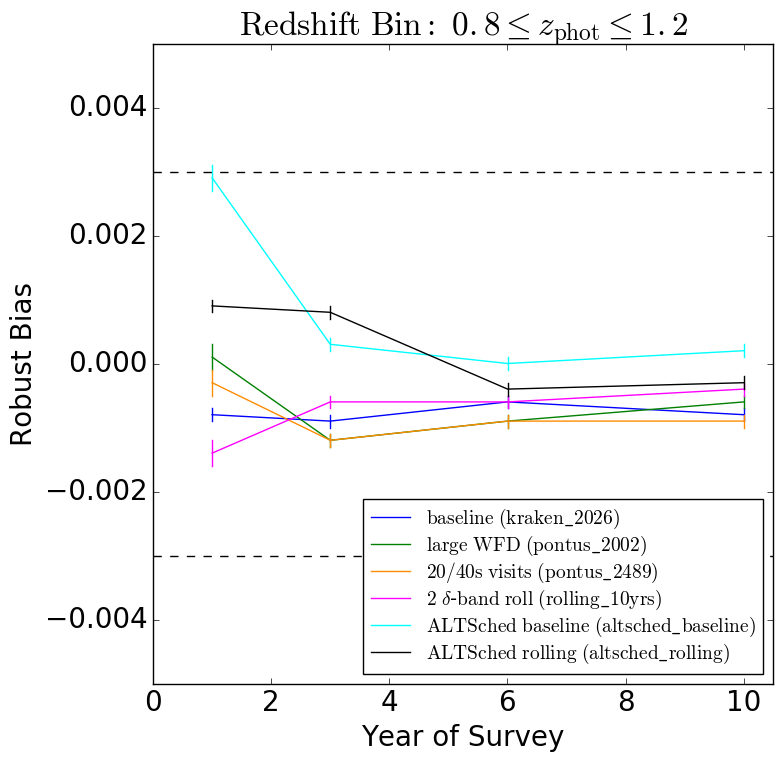
\includegraphics[width=7cm,trim={0cm 0cm 0cm 0cm},clip]{figures/zbin1_bias.png}
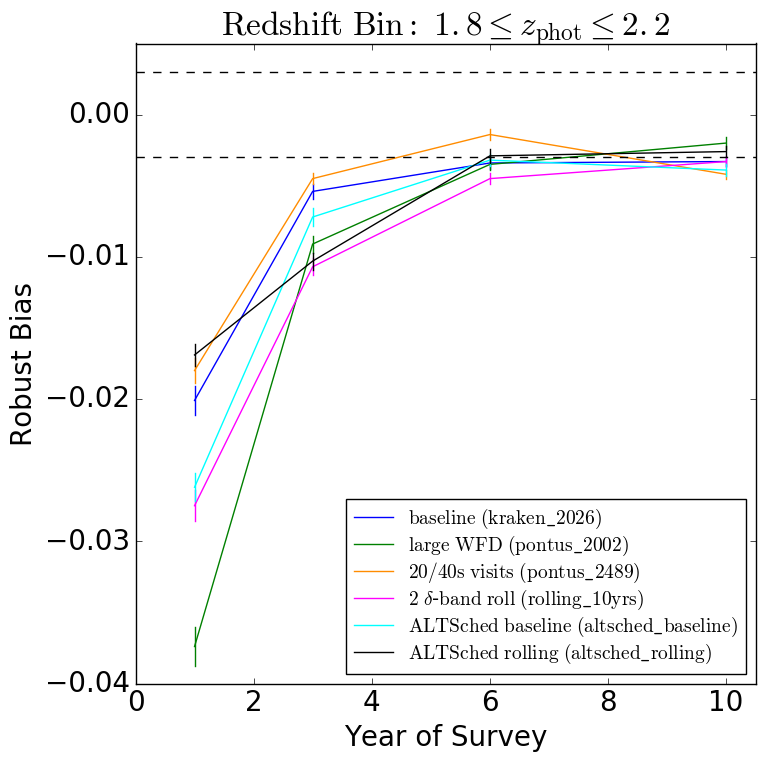
\includegraphics[width=7cm,trim={0cm 0cm 0cm 0cm},clip]{figures/zbin2_bias.png}
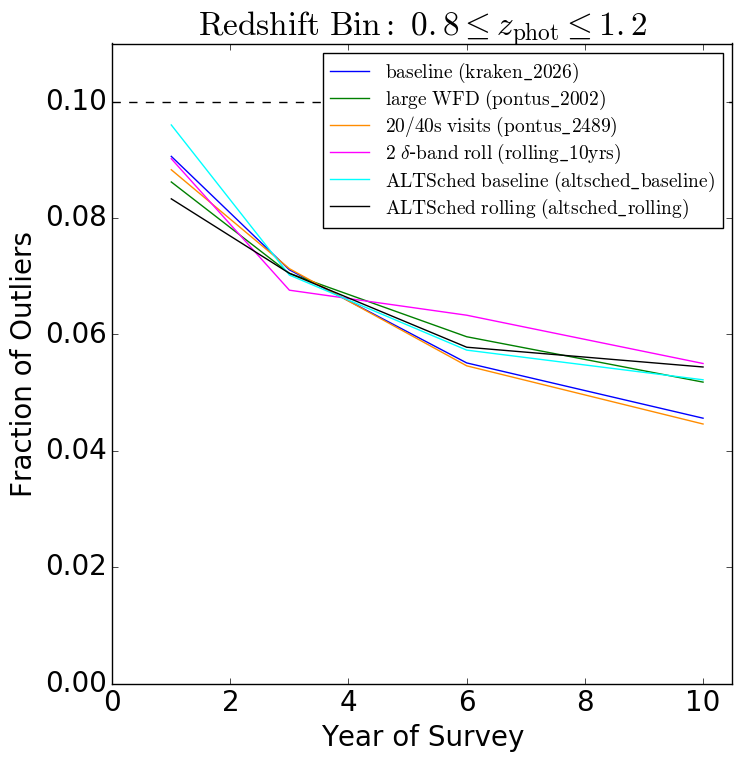
\includegraphics[width=7cm,trim={0cm 0cm 0cm 0cm},clip]{figures/zbin1_fout.png}
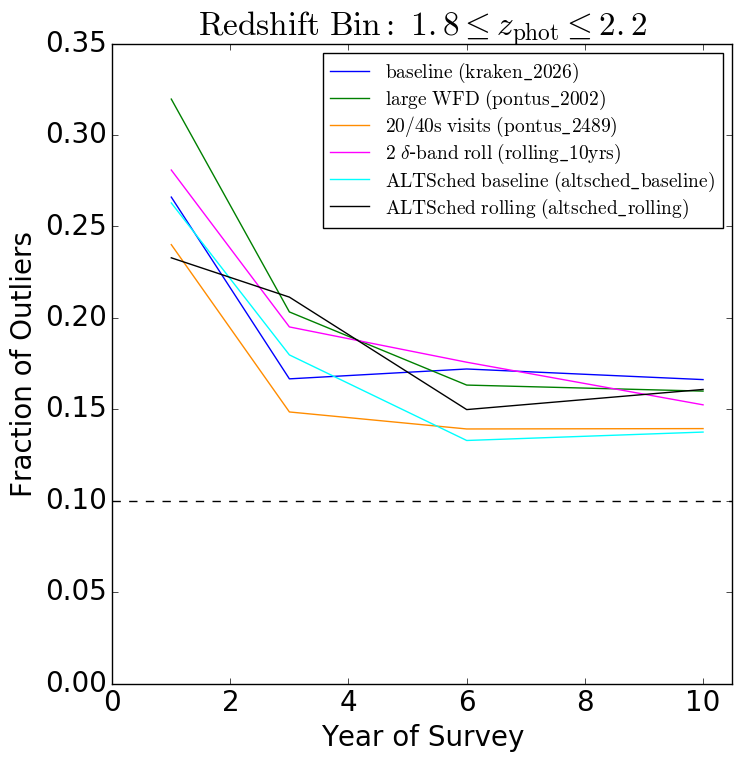
\includegraphics[width=7cm,trim={0cm 0cm 0cm 0cm},clip]{figures/zbin2_fout.png}
\caption{Statistical measures of robust standard deviation (from the IQR; top), robust bias (middle), and fraction of outliers (bottom) as a function of the LSST survey year, for bins of photometric redshift $0.8 \leq z_{\rm phot} \leq 1.2$ (left column) and  $1.8 \leq z_{\rm phot} \leq 2.2$ (right column). Note that the $y$-axes are not matched between columns. Results are presented for the baseline ({\tt kraken\_2026}; blue), large WFD area with declinations including  $-78<\delta<+18$ degrees ({\tt pontus\_2002}; green), the ``many visits" strategy with 40/20 second exposures in $u$/$grizy$ filters ({\tt pontus\_2489}; orange), a rolling cadence with two declination bands ({\tt rolling\_10yrs}; magenta), and the {\tt ALTSched} results for a baseline (cyan) and rolling (black) cadence. Horizontal dashed line represents the LSST Science Requirement Document's target for a photo-$z$ bin of $0.3 \leq z_{\rm phot} \leq 3.0$. \label{fig:evol}}
\end{center}
\end{figure}

\begin{table}\label{tab:zbins}
\caption{Relative Robust Standard Deviation of the Simulated Photometric Redshifts}
\begin{center}
\begin{tabular}{|l|cc|cc|cc|cc|}
\hline
{\tt OpSim}/{\tt ALTSched} Run & \multicolumn{2}{|c|}{Year 1} & \multicolumn{2}{|c|}{Year 3} & \multicolumn{2}{|c|}{Year 6} & \multicolumn{2}{|c|}{Year 10} \\ 
\multicolumn{1}{|r|}{$z_{\rm phot}$ Bin:} & 0.3--1.5 & 1.5--3.0 & 0.3--1.5 & 1.5--3.0 & 0.3--1.5 & 1.5--3.0 & 0.3--1.5 & 1.5--3.0 \\
\hline
baseline (kraken\_2026)                 & 1.95 & 4.07 & 1.42 & 2.58 & 1.15 & 2.05 & {\bf 1.00} & 1.83 \\ 
large WFD (pontus\_2002)                & 2.04 & 4.83 & 1.54 & 3.13 & 1.28 & 2.37 & 1.10 & 1.98 \\
many visits (pontus\_2489)              & 1.96 & 4.03 & 1.42 & 2.48 & 1.17 & 2.03 & 1.02 & 1.73 \\
$2$ $\delta$-band roll (rolling\_10yrs) & 1.87 & 3.92 & 1.53 & 3.04 & 1.24 & 2.29 & 1.10 & 1.98 \\
{\tt ALTSched} baseline                       & 1.98 & 4.35 & 1.52 & 2.89 & 1.25 & 2.28 & 1.11 & 1.95 \\
{\tt ALTSched} rolling                        & 1.69 & 3.38 & 1.55 & 3.08 & 1.26 & 2.35 & 1.11 & 1.93 \\
\hline
\end{tabular}
\end{center}
\end{table}


% % % % % % % % % % % % % % % % % % % % % % % % % % % % %
\subsection{Summary of Key Results} \label{ssec:pz_execsum}

\noindent
1. Most of the {\tt OpSim} and {\tt ALTSched} observing strategies result in a similar evolution of the median photometric depth in each filter, except: (a) when the WFD area is extended to $24,700$ square degrees (degraded photometric depth); (b) when 20/40 second visits are used for $grizy$/$u$ filters (improved photometric depth in $u$-band); or (c) when a rolling cadence is adopted (improved photometric depth of observed area in year 1). Photo-$z$ results are only simulated for these strategies that deliver a different photometric depth compared to the baseline cadence.

\medskip \noindent
2. The observing strategy in which 20/40 second visits are used for $grizy$/$u$ is the only one which exhibits improvements to the photo-$z$ quality over the baseline cadence option.

\medskip \noindent
3. The {\tt OpSim} and {\tt ALTSched} simulations offer essentially equivalent photo-$z$ results, with the exception that the {\tt ALTSched} rolling cadence delivers a significant improvement in year 1 only. We attribute the latter to the fact that the {\tt ALTSched} rolling cadence does not allocate any visits to the deprioritized declination band, whereas {\tt OpSim}'s rolling cadence allows it $25\%$ of the baseline number of visits.


% Need these new commands to compile:
%\newcommand{\todo}[2]{\textcolor{red}{\textbf{TODO (#1): #2}}}
%\newcommand{\comment}[1]{\textcolor{blue}{\textbf{#1}}}


\newcommand{\altsched}{\textcolor{magenta}{alt\_sched}} 
\newcommand{\altschedrolling}{\textcolor{blue}{alt\_sched\_rolling}}
\newcommand{\baseline}{\textcolor{orange}{baseline2018a}}
\newcommand{\colossusfour}{\textcolor{orange}{colossus\_2664}}
\newcommand{\colossusfive}{\textcolor{orange}{colossus\_2665}}
\newcommand{\colossusseven}{\textcolor{magenta}{colossus\_2667}}
\newcommand{\krakentwosix}{\textcolor{orange}{kraken\_2026}}
\newcommand{\krakenfive}{\textcolor{orange}{kraken\_2035}}
\newcommand{\krakenthreesix}{\textcolor{blue}{kraken\_2036}}
\newcommand{\krakentwo}{\textcolor{orange}{kraken\_2042}}
\newcommand{\krakenfour}{\textcolor{magenta}{Kraken\_2044}}
\newcommand{\mothrafive}{\textcolor{blue}{mothra\_2045}}
\newcommand{\mothranine}{\textcolor{blue}{Mothra\_2049}}
\newcommand{\nexusseven}{\textcolor{blue}{Nexus\_2097}}
\newcommand{\pontuszerozerotwo}{\textcolor{orange}{Pontus\_2002}}
\newcommand{\pontusfivezerotwo}{\textcolor{orange}{pontus\_2502}}
\newcommand{\pontusnine}{\textcolor{magenta}{pontus\_2489}}
\newcommand{\pontusfivezerosix}{\textcolor{magenta}{pontus\_2506}}
\newcommand{\rollingmixopsim}{\textcolor{magenta}{rolling\_mix\_10yrs\_opsim}}
\newcommand{\rollingopsim}{\textcolor{orange}{rolling\_10yrs\_opsim}}


\section{Strong Lensing}
\textit{Authors: Simon Huber\footnote{shuber@mpa-garching.mpg.de}, Sherry H.~Suyu\footnote{suyu@mpa-garching.mpg.de}, Tanja Petrushevska\footnote{tanja.petrushevska@ung.si}, Timo Anguita, Phil Marshall, Lynne Jones }

\

The Hubble constant $H_0$ is one of the key parameters to describe the
universe. Current observations of the CMB (cosmic microwave
background) assuming a flat $\Lambda$CDM cosmology and the standard
model of particle physics yield $H_0 = 67.36 \pm 0.54 \, {\rm km\,s^{-1}\,Mpc^{-1}}$
\citep{Planck:2018vks} which is in tension with $H_0 =
73.52 \pm
  1.62 \, {\rm km\,s^{-1}\,Mpc^{-1}}$ from the local distance ladder
\citep{Riess:2016jrr,Riess:2018byc}. In order to verify or refute this
$3.6 \sigma$ tension, further independent methods are needed. 

One such method is lensing time delay cosmography which can determine
$H_0$ in a single step. The basic idea is to measure the time delays
between multiple images of a strongly lensed variable source
\citep{Refsdal:1964}. This time delay, in combination with mass
profile reconstruction of the lens and line-of-sight mass structure,
yields directly a ``time-delay distance'' that is inversely
proportional to the Hubble constant ($t \propto D \propto
H_0^{-1}$). Applying this method to four lensed quasar systems, the
H0LiCOW collaboration \citep{Suyu:2016qxx} together with the
COSMOGRAIL collaboration
\citep[e.g.]{Eigenbrod:2005ie,2013Tewes,2017Courbin} measured $H_0 =
72.5^{+2.1}_{-2.3} \,{\rm km\,s^{-1}\,Mpc^{-1}}$ in flat
$\Lambda$CDM \citep{Birrer:2018vtm}, which is in agreement with the
local distance ladder and higher than CMB measurements.  Another
promising approach goes back to the initial idea of
\cite{Refsdal:1964} using lensed supernovae (LSNe) instead of quasars
for time-delay cosmography. Here we investigate the prospects of using
LSST for measuring time delays of both lensed supernovae and lensed
quasars.

\subsection{Supernovae Lensed by Galaxies}
\textit{Contributors: Simon Huber, Sherry H.~Suyu}

\

Even though the number of LSNe is significantly lower than the number of
lensed quasars, LSNe have some important advantages. First 
the sharp rise
and decline of SN light curves make time-delay measurements easier and possible
on shorter time scales in comparison to stochastically varying quasars. Second LSNe Ia are very promising
to break the model degeneracies \citep{Schneider:2013wga} in two
independent ways using dynamics \citep{Barnabe2011,2017:Yildirim} or
the standard candle nature of SNe Ia.  

So far only two systems with resolved
multiple images have been observed, namely SN ``Refsdal''
\citep{Kelly:2015xvu,Kelly:2015vjq} and iPTF16geu
\citep{Goobar:2016uuf}. But LSST will play a key role to detect many
more LSNe. At the moment we expect to find approximately $50$ resolved
LSNe Ia \citep{Oguri:2010} or $900$ in total \citep{Goldstein:2017bny}
over the 10 year survey. No other survey is capable of providing such
high numbers.

The goal of this section is to evaluate different
cadences for LSNe time-delay measurements. For this purpose we have investigated
20 different observing strategies: 15 from the call for whitepapers
(baseline2018a, kraken\_2026, colossus\_2665, pontus\_2002,
colossus\_2664, colossus\_2667, pontus\_2489, kraken\_2035,
mothra\_2045, pontus\_2502,
kraken\_2036, kraken\_2042, kraken\_2044, mothra\_2049, nexus\_2097)\footnote{\url{http://astro-lsst-01.astro.washington.edu:8080/}},
pontus\_2506 which is a cadence from Tiago Ribeiro doing the revisit
after 30 minutes in different filters, alt\_sched and
alt\_sched\_rolling from Daniel Rothchild and collaborators\footnote{\url{http://altsched.rothchild.me:8080/}}, and rolling\_10yrs\_opsim and rolling\_mix\_10yrs\_opsim from Peter Yoachim\footnote{https://github.com/yoachim/SLAIR\_runs}. 

For a better interpretation we subdivide the strategies into three categories: 

(1) \textcolor{orange} {baseline like in terms of inter-night gap and cumulative season length} (mean values), (2) \textcolor{blue}{shorter inter-night gap, shorter cumulative season length} and (3) \textcolor{magenta}{shorter inter-night gap, baseline like cumulative season length}. In addition cadences with a \textbf{large nominal WFD footprint} start with a capital letter.

The mean cumulative season length and mean inter-night gap for the categorization are shown in Figure \ref{fig:cadences categories}. The results are calculated from simulations of the 20 observing strategies by taking the mean of all fields under consideration. The mean cumulative season length is calculated by taking the mean of the summed up season length over all seasons. For the inter-night gap the revisits of a field within hours in the same filter are summarized into a single visit. We look at two different cases. The first case considers 719 LSST fields where all lie in the WFD survey. These fields are picked by taking all fields with center in $\mathrm{Dec} \in [-58,-2] \, \si{\deg}$ and  $\mathrm{RA} \in [0,120] \cup [330,360] \, \si{\deg}$, where all DDFs are excluded. By choice the Galactic Plane, the South Celestial Pole and the Northern Ecliptic are completely excluded and the 719 fields represent only the WFD survey and are used to classify the cadences. For comparison we consider in the second case all 5292 LSST fields covering the entire sky, where we only take into account those fields of the 5292 where observations are taken.


\begin{figure}
\centering
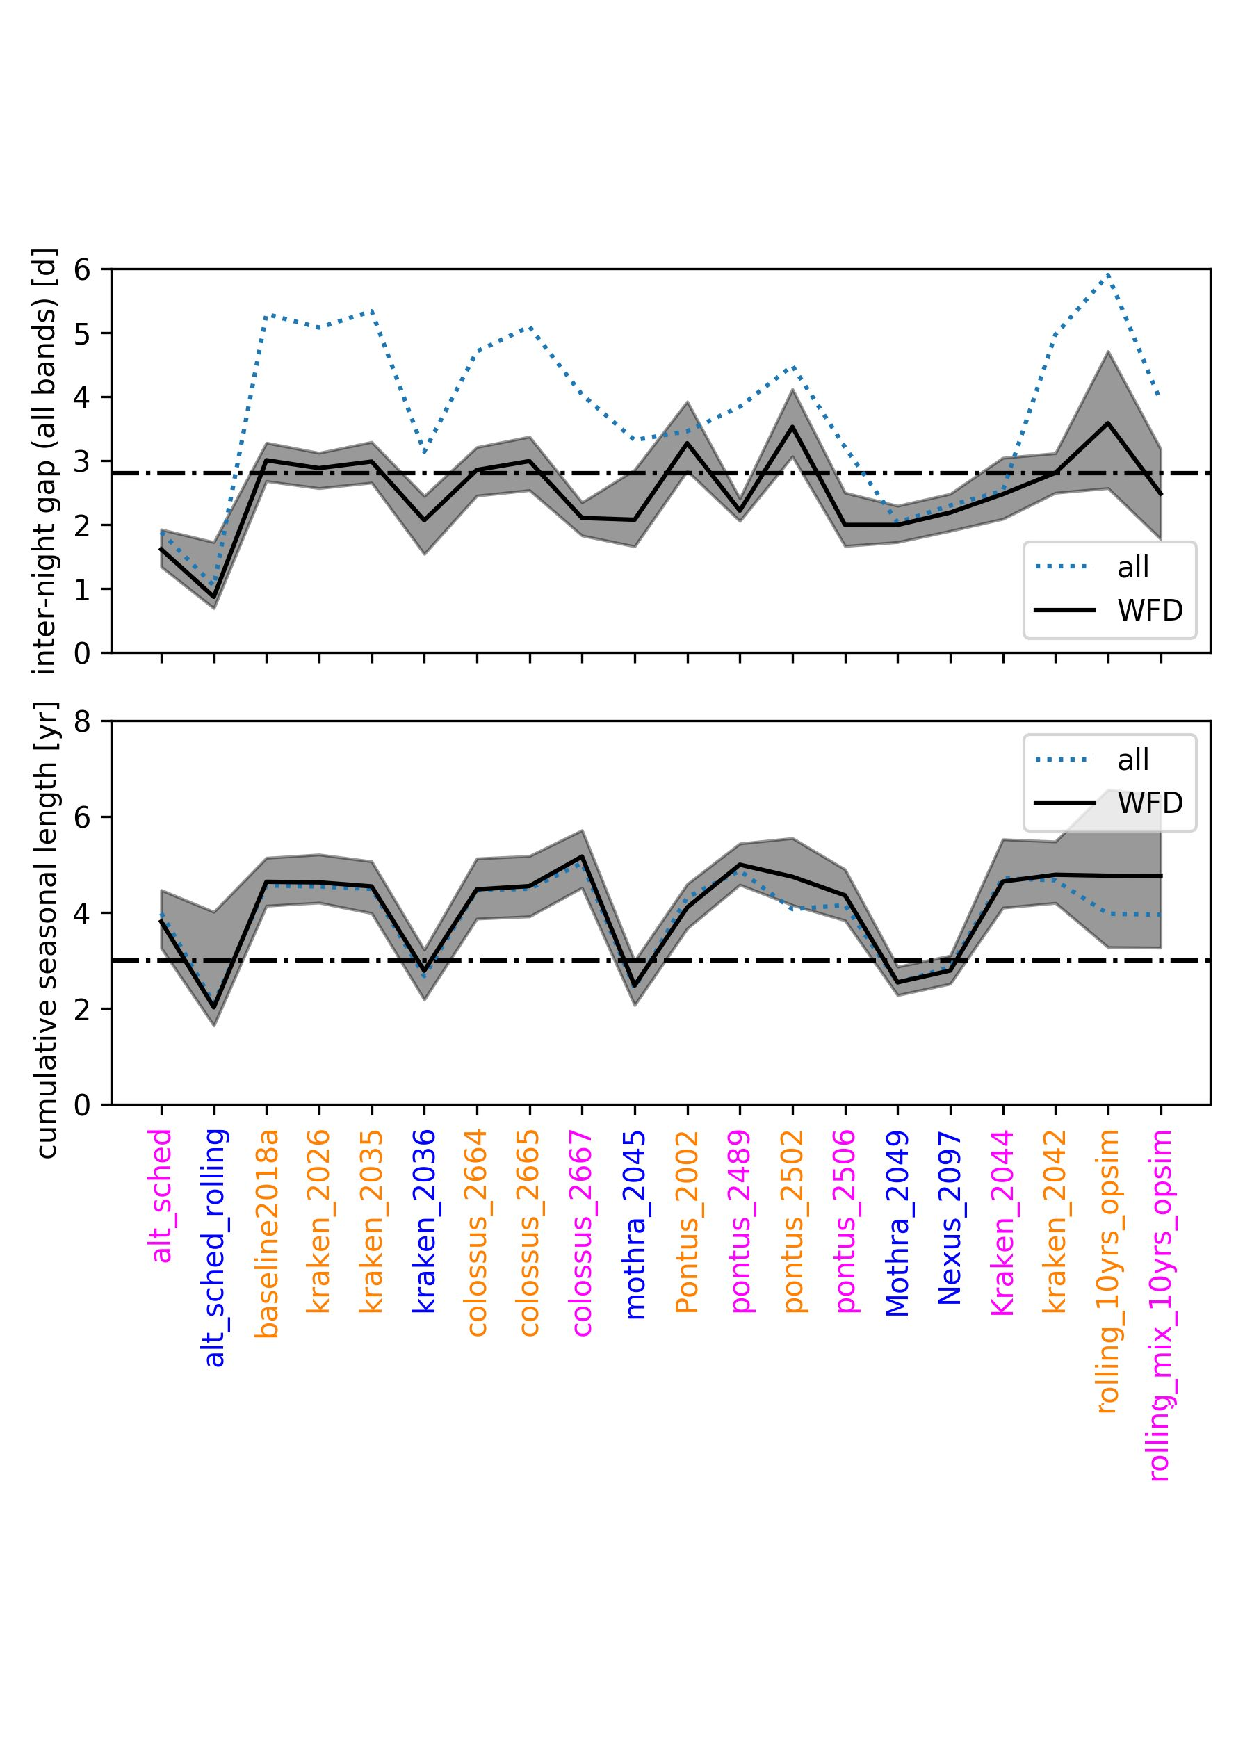
\includegraphics[scale=0.6]{figures/sl_cadences.pdf}
\caption{The mean inter-night gap (upper panel) and mean cumulative season length (lower panel) for 20 different observing strategies for two cases. The first case ("WFD" in solid black) considers 719 LSST fields, which all lie in the WFD survey. The shaded region encloses the 99th percentile of the WFD fields. The second case ("all" in dotted blue) considers all LSST fields (5292) where observations are taken. In the upper panel cadences with the black line below the black dot-dashed line are those with a significantly better inter-night gap than the baseline cadence (magenta and blue strategies). By looking at the lower panel these are subdivided into strategies with a cumulative season length similar to the baseline cadence (magenta) and a significantly worse cumulative season length (blue). Observing strategies in orange have a baseline like mean inter-night gap and mean cumulative season length.}
\label{fig:cadences categories}
\end{figure}

To simulate observations randomly, we have used 202
mock LSNe Ia from the OM 10 catalog \citep{Oguri:2010},
and produced the light curves for the mock SNe images with
the spherically symmetric SN Ia W7 model \citep{1984:Nomoto}
calculated with ARTIS (Applied Radiative Transfer In Supernovae)
\citep{Kromer:2009ce} in combination with magnifications maps from
GERLUMPH \citep{Vernardos:2015wta} to include the effect of
microlensing similar as in \citep{Goldstein:2017bny}. We then simulate
data points for the light curves, following the observation pattern from different cadences
and uncertainties according to the LSST science book
\citep{2009:LSSTscience}. To measure the time delay from the simulated
observation we use the free knot spline optimizer from PyCS (Python
Curve Shifting) \citep{2013:Tewesb,Bonvin:2015jia}. Details of this
work will be presented in Huber et al. (in preparation).


The structure of this subsection is organized as follows. In
\ref{sec:simulation of mock data} we describe how we simulate and
evaluate the mock data and in \ref{sec:results} we present our results
where we have quantified 20 cadences for LSNe Ia.

\subsubsection{Simulating and evaluating mock data}
\label{sec:simulation of mock data}
To simulate mock data for the different cadences we have picked 10
fields in the WFD (wide fast deep survey) which are listed in Table
\ref{tab: 10 wfd fields}. For a given cadence for each of these
fields, we store the following for each visit of the field: date
(mjd), filter(s) observed, and 5-$\sigma$ depth $m_5$. Such an
observing sequence of visits is illustrated for the ``baseline2018a''
cadence in figure \ref{fig:observation patter LSST 10 year survey},
where for one field in the WFD all observations within the 10 year
survey are shown. 
%
\begin{figure}
\centering
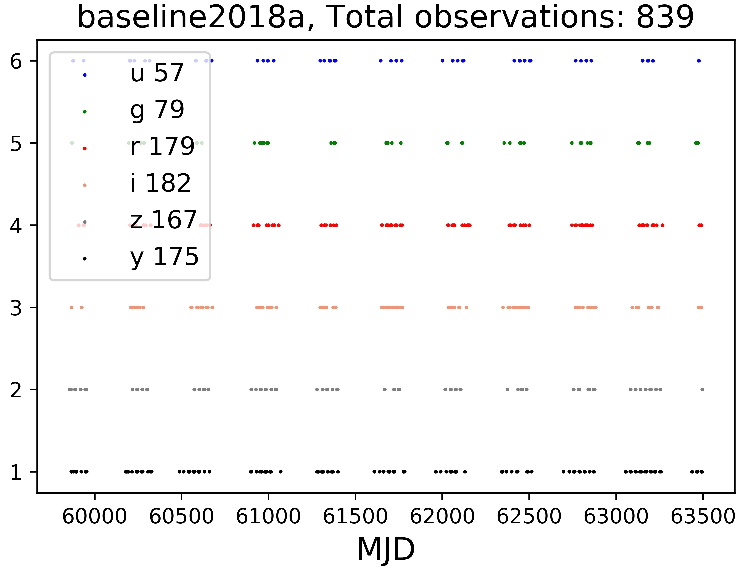
\includegraphics[scale=0.7]{figures/sl_field_number3_baseline2018a_Daniel.pdf}
\caption{This illustrates for the observing strategy ``baseline2018a'' the mjd and filter when observations are taken over the 10 year survey for field number 4 in table \ref{tab: 10 wfd fields} in the wide fast deep survey}
\label{fig:observation patter LSST 10 year survey}
\end{figure}
%
%\FloatBarrier 
To simulate observational data of a LSN system, we place randomly in
one of the 10 choosen fields from Table \ref{tab: 10 wfd fields} a
mock LSNe Ia from the OM 10 catalog, which is a mock catalog for
strong gravitational lenses \citep{Oguri:2010}. The catalog contains
about 400 LSNe Ia (The catalog is 10 times oversampled which means
that the total number of LSNe Ia is about 40) for LSST with an image
separation larger than $\SI{0.5}{\arcsec}$. For the lens model an SIE
(singular isothermal ellipsoid) \citep{Kormann:1994} is assumed and
therefore the time delay $\tau$, the convergence $\kappa$ and the
shear $\gamma$ is known for each of the multiple SNe images. By
assuming a W7 model and placing each of the SNe images randomly in the
corresponding magnification map one can calculate mock light
curves. Furthermore we place the mock system randomly in time, such
that the detection criterion applied in OM 10 is fulfilled. The
criterion is that the peak of the i-band magnitude of the fainter image
for a double or the 3rd brightest image for a quad, falls in the
observing season.
By combining this with the observing sequence, we get simulated
observations as illustrated in figure \ref{fig: simulated observation}
for a quad system. The error is calculated according to \cite[sec 3.5,
p. 67]{2009:LSSTscience}.
\begin{figure}[h!]
\centering
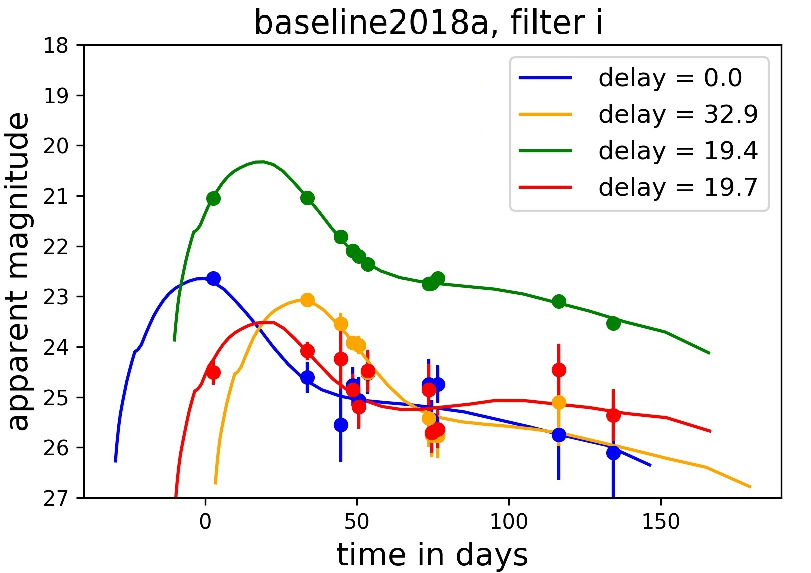
\includegraphics[scale=0.7]{figures/sl_Obsevation_number399_baseline2018a_filter_i_oversampling_00.pdf}
\caption[]{In this figure the i-band light curves of a mock quad LSNe Ia are shown. The observation sequence is for a random field in WFD survey for the cadence ``baseline2018a''.}
\label{fig: simulated observation}
\end{figure}
%
\begin{table}
\centering
\begin{tabular}{c|c|c|c|c|c|c|c|c|c|c}
field number & 1 & 2 & 3 & 4 & 5& 6 & 7 & 8 & 9 & 10  \\
\hline
RA& 0.0 & 32.1 & 65.8 & 50.9 &44.9& 125.6 & 155.0 & 207.7 & 304.3 & 327.5  \\
\hline
DEC& -7.4 & -44.2 & -7.2 & -30.0 & -50.9& -11.4 & -25.6 & -45.3 & -55.2 & -35.9  \\
\end{tabular}
\caption{The 10 fields of the wide fast deep survey, where the observation sequence for different cadences was considered.}
\label{tab: 10 wfd fields}
\end{table}
%
%\FloatBarrier

To evaluate the mock data and get a measured time delay we use the
free knot spline optimizer from PyCS (Python Curve Shifting)
\citep{2013:Tewesb,Bonvin:2015jia}. PyCS was initially developed to
measure time delays in strongly lensed quasars, and is not yet
optimised for LSNe Ia, such as fitting simultaneously multiple filters
and using SN template light curves.  Applying PyCS to individual
filter's light curves, we get a single independent time delay for each
filter.  We combine the 6 delays from the 6 LSST filters afterwards
into a single delay, but we expect more precise and accurate delays by
using multi-color fitting in the future. We also expect improvements
in delay measurements with the use of SNe Ia template instead of
splines.  

%so there are still
%some improvements for LSNe Ia, which will be implemented in the
%future. The first one is that to date multi-color time delay fitting
%is not possible, which means that we get a single independent time
%delay for each filter. We combine this 6 delays afterwards to a single
%delay, but we expect more precise and accurate delays by using
%multi-color fitting. A second improvement might be the use of SNe Ia
%templates instead of splines. This means that we do a conservative
%time delay estimate and with future improvements we might be able to
%measure time delays even better. 

To have sufficient statistics, we investigate for each cadence
strategy 202 mock LSNe Ia, where we pick 50 \% doubles and 50 \%
quads. For each of the mock systems we draw 100 random starting
configurations. A starting configuration corresponds to a random
position in the microlensing map and a random field from Table
\ref{tab: 10 wfd fields}, where it is placed randomly in one of the
observing seasons such that the detection requirement from OM 10 is
fulfilled. For each of these starting configurations we then draw 1000
different noise realizations of light curves, where we also shift the
time delays for each noise realizations randomly by $-3$ to
$\SI{3}{\day}$, to estimate uncertainties of delay measurements with
PyCS. For each realization we calculate the deviation from the true
time delay as
%
\begin{equation}
\tau_\mathrm{d} = \frac{t_\mathrm{measured} - t_\mathrm{true}}{t_\mathrm{true}}.
\label{eq: deviation from true time delay}
\end{equation}
For one strategy and double LSNe Ia, we have thus $1 {\rm (delay\ for\ the\
one\ pair\ of\ images)} \times 6 {\rm (filters)} \times 100 {\rm
(starting\ configurations)} \times 1000 {\rm (noise\ realisations)}$
time-delay deviations as in \eqref{eq: deviation from true time delay}.
%, where the 6 stands for the 6 LSST filters. 
For the 6 pairs of images for a quad system we have a sample of $6
\times 6 \times 100 \times 1000$. The resulting distribution of
time-delay deviation is investigated for each pair of images and each
filter separately. From the $100 \times 1000$ time-delay deviations we
define accuracy as the median $\tau_\mathrm{d,50}$ and precision as
$\delta = (\tau_\mathrm{d,84}-\tau_\mathrm{d,16})/2$, where
$\tau_\mathrm{d,84}$ is the 84th and $\tau_\mathrm{d,16}$ the 16th
percentile. Measuring $H_0$ with 1\% accuracy requires that the accuracy
in the delay deviation $\tau_\mathrm{d,50}$ is $<1\%$ (since $H_0 \propto
t_{\rm true}^{-1}$). Since the 6 time-delay deviations from the 6 filters are independent we combine them into a single time-delay deviation via the weighted mean. This means that in the end we have for one strategy and a mock LSNe Ia one 
\begin{equation}
\tau_\mathrm{d,50} \pm \delta
\label{eq: accuracy and precission}
\end{equation}
per pair of images.


\subsubsection{Results}
\label{sec:results}
In this section we summarize the results and quantify the 20
investigated cadences. Given that $H_0 \propto \frac{1}{t}$, where $t$
is the time delay between two images, we aim for accuracy
($\tau_\mathrm{d,50}$) smaller than 1 percent and precision ($\delta$)
smaller than 5 percent in equation \ref{eq: accuracy and precission}. The accuracy
requirement is needed for measuring $H_0$ with 1\% uncertainty, and
the precision requirement ensures that the delay uncertainty does not
dominate the overall uncertainty on $H_0$ given typical mass modeling
uncertainties of $\sim 5\%$ \citep[e.g.,][]{Suyu2018}.  A quad system is counted as successful if one of the 6 delays fulfills this requirement. 
We have investigated two different cases, first using LSST data only to measure time delays and second, using LSST as a discovering machine in combination with follow-up observations to measure delays. 
For just using LSST data we have investigated 202 mock LSNe Ia and for using LSST in combination with follow-up 100 mock systems have been investigated, where for each case 50 \% are doubles and 50 \% are quads. 
We assume follow-up observation would start 2 days 
after the third LSST data point in any filter exceeds the 5-$\sigma$ 
depth, where the follow-up is done in 3 filters (g,r,i) every second night.
The fraction of systems for which the time-delay measurement fulfills the above defined requirement is summarized in columns 3 and 5 of Table \ref{tab: quantify different observing strategies}. These numbers have to be combined with the total number of LSNe Ia we expect to detect for different strategies. We approximate the total number of LSNe Ia as

\begin{align}
\label{eq: total number of LSNe Ia from modified OM 10}
N_\mathrm{LSNe Ia, cad} = N_\mathrm{LSNe Ia, OM 10} \frac{\Omega_\mathrm{cad}}{\Omega_\mathrm{OM 10}} \frac{\bar{t}_\mathrm{eff,cad}}{t_\mathrm{eff, OM 10}}
\end{align}
%
where $N_\mathrm{LSNe Ia, OM10} = 45.7$, $\Omega_\mathrm{OM10} = \SI{20000}{\square\deg}$ and $t_\mathrm{eff, OM10}=\SI{2.5}{\year}$ from \cite{Oguri:2010}. $\bar{t}_\mathrm{eff,cad}$ is the mean effective/cumulative seasonal length for a given cadence strategy, where we have averaged over all 719 WFD fields. $\Omega_\mathrm{cad}$ is the survey area for a given observing strategy. Instead of taking the nominal values (see column 2 Table \ref{tab:LSST Survey Area for different observing strategies}) we calculate the area from fields represented by our study. These are fields with a mean cumulative season length and inter-night gap similar or even better than the 719 WFD fields, meaning: Cumulative season length ($t_\mathrm{eff}$) longer than the lower 99th percentile and inter-night gap ($t_\mathrm{gap}$) shorter than the upper 99th percentile. Further we also take into account the 5-$\sigma$ depth ($m_5$)\footnote{Here we consider only the main relevant bands g,r,i and z.}. Here we consider all fields with ($m_5+0.2 \mathrm{mag}$) greater than the lower 99th percentile of the 719 WFD fields. The relaxed 5-$\sigma$ depth is necessary in order to represent the wider areas as suggested by the nominal values. The area can then be calculated from the number of systems fulfilling the above defined criteria times the field of view of $\SI{9.6}{\square\deg}$ taking into account the overlap factor of the fields:
%
\begin{align}
\Omega_\mathrm{cad} = f_\mathrm{overlap} \cdot N_\mathrm{cad,criteria} \cdot \SI{9.6}{\square\deg},
\end{align}
where
$f_\mathrm{overlap}=\frac{5292 \cdot \SI{9.6}{\square\deg}}{4 \pi \cdot (\SI{180}{\deg}/\pi)^2} \approx 0.812.$
The calculated area is shown in column 3 of Table \ref{tab:LSST Survey Area for different observing strategies}. They still represent the wider areas as suggested by the nominal values, but are more representative in terms of delay measurements than the nominal areas because they contain observational constraints on cumulative season length, inter-night gap and 5-$\sigma$ depth\footnote{The 0.2 mag difference in the 5-$\sigma$ depth would reduce for the LSST + follow-up case the number of detected systems by a few percents, whereas, it does not matter for the case of using LSST only.}.

\begin{table}
\centering

\begin{tabular}{c|c|c|c}                                                                                               
& $\Omega_\mathrm{nom}$ & $\Omega_\mathrm{cad}$ &  $(\Omega_\mathrm{cad}-\Omega_\mathrm{nom})/\Omega_\mathrm{nom} [\%]$ \\
\hline
\altsched          &  18000 &  17703 &  -1.6 \\
\altschedrolling   &  18000 &  20463 &  13.7 \\
\baseline          &  18000 &  17306 &  -3.9 \\
\colossusfour      &  18000 &  18202 &   1.1 \\
\colossusfive      &  18000 &  18475 &   2.6 \\
\colossusseven     &  18000 &  17797 &  -1.1 \\
\krakentwosix      &  18000 &  17119 &  -4.9 \\
\krakenfive        &  18000 &  17680 &  -1.8 \\
\krakenthreesix    &  18000 &  17719 &  -1.6 \\
\krakentwo         &  18000 &  17828 &  -1.0 \\
\krakenfour        &  24700 &  24010 &  -2.8 \\
\mothrafive        &  18000 &  16417 &  -8.8 \\
\mothranine        &  24700 &  21874 & -11.4 \\
\nexusseven        &  24700 &  20471 & -17.1 \\
\pontuszerozerotwo &  24700 &  22926 &  -7.2 \\
\pontusnine        &  18000 &  17758 &  -1.3 \\
\pontusfivezerotwo &  18000 &  17602 &  -2.2 \\
\pontusfivezerosix &  18000 &  18132 &   0.7 \\
\rollingopsim      &  18000 &  18148 &   0.8 \\
\rollingmixopsim   &  18000 &  18132 &   0.7 \\
\end{tabular} 
 \caption{Survey areas for different observing strategies. The second column contains the nominal values and the third column shows the area used for Equation \ref{eq: total number of LSNe Ia from modified OM 10} taking into account observational constraints (see text). The forth column shows the deviation from the nominal values in percent.}
 \label{tab:LSST Survey Area for different observing strategies}
\end{table}




The results in terms of total number of LSNe Ia for the investigated cadences are shown in column 6 of Table \ref{tab: quantify different observing strategies}, where we see that for most of the rolling cadences (blue strategies) fewer LSNe Ia will be detected, because of the shorter cumulative season lengths $\bar{t}_\mathrm{eff,cad}$. The total number depends on the selection criteria assumed in \cite{Oguri:2010}. If we relax on the criteria like the image separation these numbers will be higher, but the order of the strategies will be unchanged.

Columns 2 and 4 in Table \ref{tab: quantify different observing strategies} contain the total number of LSNe Ia where the delay can be measured with accuracy $<$ 1 \% and precision $<$ 5 \% over the 10 year survey. For the case of using only LSST data, we see that even for the best strategies we will just have
a few systems where time-delay measurements are possible. Follow-up observations are therefore necessary to
increase the number of LSNe Ia with delays as shown in column 2 of Table \ref{tab: quantify different observing strategies}. These results are also more qualitatively summarized in Table \ref{tab: favoured strategies}

To summarize, for our science case of measuring time delays from as many lensed SNe as possible, it would be more effective to use LSST as a discovering machine with additional follow-up, instead of relying on LSST completely for the delay measurements. From our investigations we find that long cumulative seasonal lengths $\bar{t}_\mathrm{eff,cad}$ and a more frequent sampling are important. To go more into detail, we request for 10 seasons with a season length of 170 days or longer. Rolling cadences are clearly disfavored, because their shortened cumulative season lengths lead to overall a more negative impact on the number of LSNe Ia with delays, compared to the gain from the increased sampling frequency\footnote{rolling\_mix\_10\_yrs\_opsim has a cumulative season length close to baseline2018a and does the revisit in different filters. It is therefore the only rolling cadence performing better than the baseline cadence.}. To improve the sampling, single visits per night would be helpful. Since this will make the science case of fast-moving transients impossible we suggest doing one revisit within a night but in a different band than the first visit. Further improvements are the replacement of $2 \times \SI{15}{\s}$ exposure by $1 \times \SI{30}{\s}$ for an increased efficiency and redistributing some of the visits in y band to g, r, i and z.
%of their shorter cumulative season lengths $\bar{t}_\mathrm{eff,cad}$ although they improve the sampling. Therefore we reject to improve on one of the 3 parameters our science case is mostly sensitive to, by worsen at the same time one of the others significantly. 
%

Further \cite{Goldstein:2018bue} performed detailed simulations of the gLSN population using a completely independent technique and pipeline and reached similar conclusions to the ones presented here: rolling cadences are strongly disfavored, and wide-area, long-season surveys with well sampled light curves are optimal.


\begin{table}
\centering
\begin{tabular}{c|cc|cc|c}
\multicolumn{1}{c}{}& \multicolumn{2}{c}{\textbf{LSST + follow-up}}  & \multicolumn{2}{c}{\textbf{LSST only}} & \multicolumn{1}{c}{ } \\

& total  & total   & total  & total  & total \\
& number  & fraction  & number  & fraction  & number \\
&  with & with & with& with & of\\
& delays & delays& delays& delays&LSNe Ia\\
\hline
\krakenfour        &  27.7 &  27.2 &  5.9 &   5.8 &  102.0 \\
\colossusseven     &  27.5 &  32.7 &  7.1 &   8.4 &   84.0 \\
\altsched          &  21.8 &  35.3 &  7.9 &  12.8 &   61.7 \\
\pontusfivezerosix &  20.1 &  27.8 &  6.1 &   8.4 &   72.2 \\
\krakentwo         &  19.7 &  25.2 &  4.5 &   5.8 &   78.0 \\
\pontusnine        &  19.3 &  23.8 &  6.0 &   7.4 &   81.1 \\
\rollingmixopsim   &  18.9 &  23.8 &  7.6 &   9.5 &   79.4 \\
\krakentwosix      &  18.7 &  25.8 &  3.5 &   4.8 &   72.4 \\
\pontuszerozerotwo &  18.1 &  21.0 &  1.2 &   1.4 &   86.1 \\
\colossusfive      &  17.2 &  22.4 &  2.9 &   3.7 &   76.8 \\
\baseline          &  16.5 &  22.4 &  2.7 &   3.7 &   73.4 \\
\colossusfour      &  15.7 &  21.0 &  3.1 &   4.1 &   74.6 \\
\krakenfive        &  15.5 &  21.0 &  2.0 &   2.7 &   73.4 \\
\altschedrolling   &  13.7 &  35.9 &  6.3 &  16.5 &   38.0 \\
\pontusfivezerotwo &  13.5 &  17.7 &  1.0 &   1.4 &   76.3 \\
\nexusseven        &  12.5 &  23.8 &  2.5 &   4.8 &   52.3 \\
\mothranine        &  12.2 &  23.8 &  2.4 &   4.7 &   51.0 \\
\rollingopsim      &  11.9 &  14.9 &  5.4 &   6.8 &   79.8 \\
\krakenthreesix    &  11.4 &  25.2 &  2.1 &   4.7 &   45.2 \\
\mothrafive        &  10.4 &  27.9 &  2.3 &   6.1 &   37.3 \\


\end{tabular}
\caption{This table quantifies 20 different cadence strategies for measuring time delays in LSNe Ia. The second and third column consider LSST as a discovery machine in combination with follow-up observations in 3 filters (g,r,i) every second night. We assume follow-up observation would start 2 days after the third LSST data point in any filter exceeding the 5-$\sigma$ depth. In the fourth and fifth column only LSST data is used to measure time delays. The sixth column shows the total amount of LSNe Ia (69 \% doubles and 31 \% quads) calculated via \eqref{eq: total number of LSNe Ia from modified OM 10}. The columns "total fraction with delays" contain the fraction of the  investigated mock LSNe Ia where the time delay could be measured with accuracy better than 1 percent and precision better than 5 percent. We have investigated 100 mock systems for LSST + follow-up and 202 mock systems for the case where only LSST data is used. The columns "total number with delays" combine the columns "total fraction with delays" with the column "total number of LSNe Ia". Since for LSST only, the total numbers with delays are very low, we advocate using LSST as a discovering machine with observational follow up. Therefore the second column is the relevant one to quantify different cadences. For a more qualitative conclusion see Table \ref{tab: favoured strategies}.}
\label{tab: quantify different observing strategies}
\end{table}
%
\begin{table}
\centering
\begin{tabular}{c|c|c|c}
& good with obs.   &  favored with . \\
& follow-up in addition to LSST  & LSST data only \\
\hline
\krakenfour        &  x &  x \\
\hline
\colossusseven     &  x &  x \\
\hline
\altsched          &  x &  x \\
\hline
\pontusfivezerosix &  x &  x \\
\hline
\krakentwo         &  x &   \\
\hline
\pontusnine        &  x &  x \\
\hline
\rollingmixopsim   &  x &  x \\
\hline
\krakentwosix      &  x &  \\
\hline
\pontuszerozerotwo &  x &  \\
\hline
\colossusfive      &  x &   \\
\hline
\baseline          &  x &  \\
\hline
\colossusfour      &  &  \\
\hline
\krakenfive        &  &   \\
\hline
\altschedrolling   &  &  x \\
\hline
\pontusfivezerotwo &  &   \\
\hline
\nexusseven        &   &   \\
\hline
\mothranine        &  &   \\
\hline
\rollingopsim      & &  x \\
\hline
\krakenthreesix    &  &   \\
\hline
\mothrafive        &  &  \\

\end{tabular}
\caption{This table ranks 20 different cadences for the scenarios combining LSST with follow-up and using LSST data only. Cadences marked with a "x" are good for the given scenario, where unmarked ones are disfavored.}
\label{tab: favoured strategies}
\end{table}
%
\FloatBarrier
\subsection{Supernovae Lensed by Galaxy Clusters}
\textit{Contributor: Tanja Petrushevska}

\

Here, we focus on prospects of observing supernovae which are lensed by known galaxy clusters. High-z galaxies that appear as multiple images in the cluster field can host supernova explosions \citep{2015Sci...347.1123K, 2016ApJ...819L...8K}. Strongly lensed supernovae by galaxy clusters not only can be used as tools to examine both global cosmology, but also the local environment of the cluster lenses \citep{2014ApJ...786....9P,2014MNRAS.440.2742N, 2015ApJ...811...70R}. Cluster lensing time scales are typically much longer and the microlensing effects are almost negligible, which makes their measurement potentially more feasible, especially if the lens potential is well studied and the predicted time delays have small uncertainties. We calculate the expected number of supernovae Ia in the multiply lensed background galaxies by using the six Hubble Frontier Fields clusters \citep{2017ApJ...837...97L}  (Abell 2744, MACS J0416.1-2403, MACS J0717.5+3745, MACS J1149.5+2223, Abell S1063 and Abell 370) and Abell 1689. These clusters have been extensively studied, and given the good quality data, well constrained magnification maps and time delays can be obtained from the lensing models (\cite{2016A&A...594A..54P, 2018A&A...614A.103P}, Petrushevska et al. 2018, in press). We only considered the multiply imaged galaxies that have a spectroscopic redshift. To obtain better image depth, we combine the images that are taken closer than 5 days in time. We note that these are a lower limits, since we have only considered few clusters and the galaxies with spectroscopic redshift. For this science case, the most important bands are i, z and y. Since most of the light of nearby SNe is in the optical bands, these filters are optimal for finding high-z SNe, as their light is redshifted to the longer wavelengths. For the details regarding the estimates presented in this section, we refer to our work (\cite{2018A&A...614A.103P,2016A&A...594A..54P}, Petrushevska et al. 2018, in press). The results are presented in Figure \ref{?}. We confirm independently the conclusions from the previous section. Furthermore, our general recommendation would be, in order to optimise the sensitivity to high-redshift SNe with multiple images in galaxy cluster fields, to obtain better image depth in the reddest bands (i, z and y) . This can also be obtained by co-adding images from visits closely separated in time.

\begin{figure}
\centering
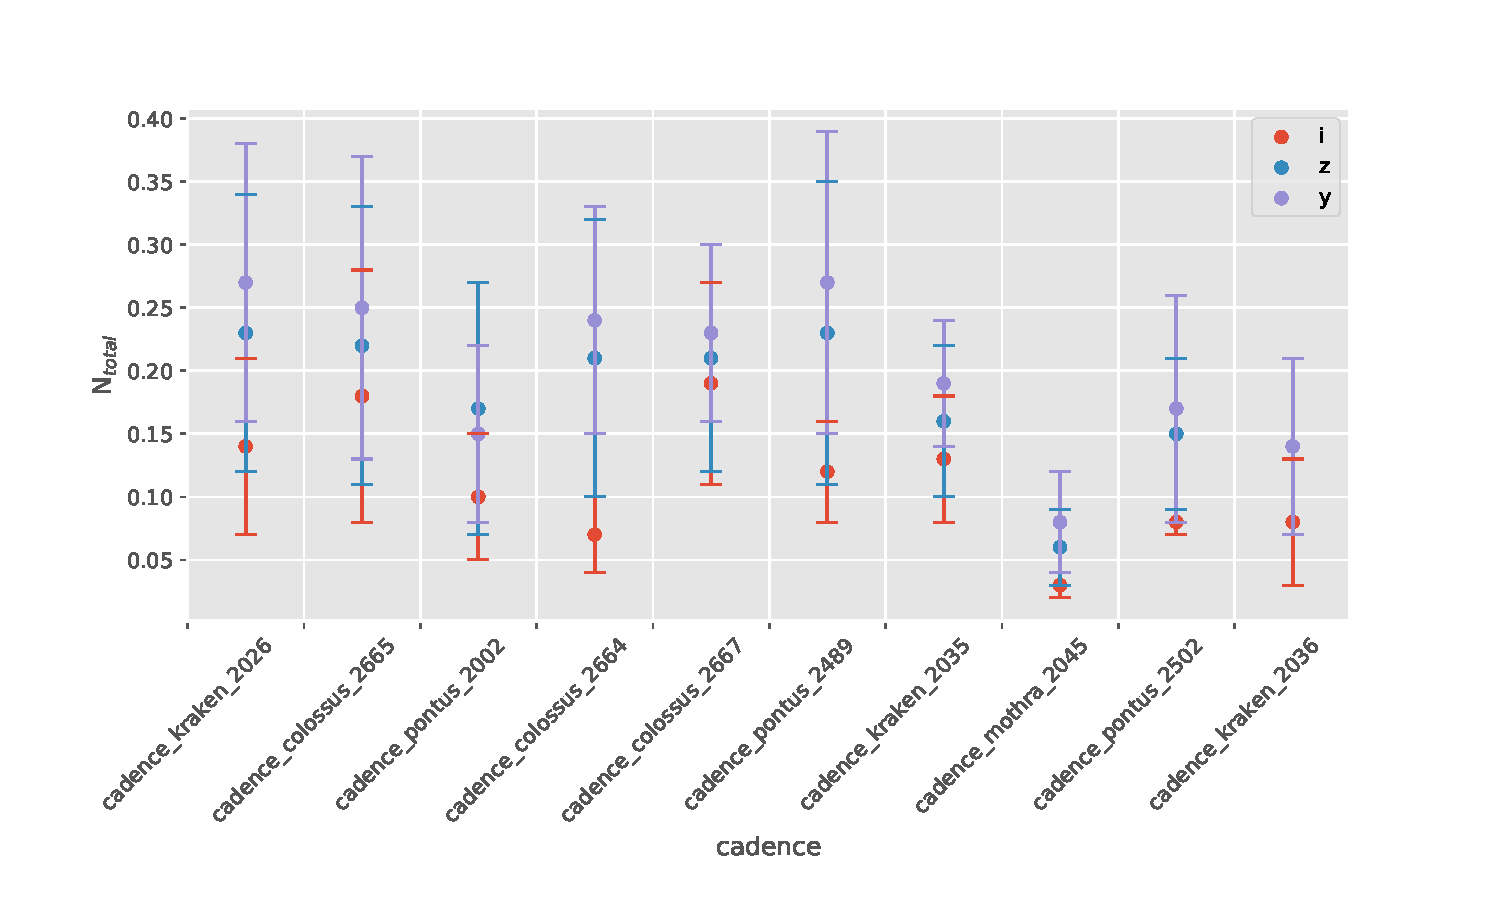
\includegraphics[scale=0.65]{figures/sl_galaxy_lensing.pdf}\caption{The expected total number of strongly lensed SNe Ia arising from the multiply imaged galaxies in the Hubble Frontier Fields and Abell 1689 in function of the observing strategy. \todo{Tanja}{include new cadences and do same estimates for CC SNe*}}
\end{figure}


\subsection{Lensed Quasars\footnote{Summarized and updated version of  \citep[Cosmology chapter of][]{LSSTScienceCollaboration2017}}}
\textit{Contributors: Phil Marshall, Timo Anguita, Lynne Jones}


The goal of this section is to evaluate the precision we can achieve in measuring time delays in strongly lensed AGN, and as such, the precision on the measurement of the Hubble constant from all systems with measured time delays.

Anticipating that the time delay accuracy would depend on night-to-night
cadence, season length, and campaign length, we carried out a large
scale simulation and measurement program that coarsely sampled these
schedule properties. In \cite{Liao2015}, we simulated 5 different
light curve datasets, each containing 1000 lenses, and presented them to
the strong lensing community in a ``Time Delay Challenge.'' These 5
challenge ``rungs'' differed by their schedule properties. Focusing on the best challenge
submissions made by the community, we derived a simple power law model
for the variation of each of the time delay accuracy, time delay
precision, and useable sample fraction, with the schedule properties
cadence, season length and campaign length. They are
given by the following equations:

\begin{align}
|A|_{\rm model} &\approx 0.06\% \left(\frac{\rm cad} {\rm 3 days}  \right)^{0.0}
\left(\frac{\rm sea}  {\rm 4 months}\right)^{-1.0}
\left(\frac{\rm camp}{\rm 5 years} \right)^{-1.1}  \notag \\
P_{\rm model} &\approx 4.0\% \left(\frac{\rm cad} {\rm 3 days}  \right)^{ 0.7}
\left(\frac{\rm sea}  {\rm 4 months}\right)^{-0.3}
\left(\frac{\rm camp}{\rm 5 years} \right)^{-0.6}  \notag \\
f_{\rm model} &\approx 30\% \left(\frac{\rm cad} {\rm 3 days}  \right)^{-0.4}
\left(\frac{\rm sea}  {\rm 4 months}\right)^{ 0.8}
\left(\frac{\rm camp}{\rm 5 years} \right)^{-0.2} \notag 
\end{align}

All three of these diagnostic metrics would, in an ideal world, be
optimized: this could be achieved by decreasing the night-to-night
cadence (to better sample the light curves), extending the observing
season length (to maximize the chances of capturing a strong variation
and its echo), and extending the campaign length (to increase the number
of effective time delay measurements).

The quantity of greatest scientific interest is the {\it accuracy in
	cosmological parameters}: this could be computed as follows. Setting a
required accuracy threshold  defines the available number of lenses,
which in turns gives us the mean precision per lens there. Combining the
whole sample, we would get the error on the weighted mean time delay, as
used by \cite{Coe2009}. This uncertainty, which scales as one
over the square root of the number of available lenses,  can be roughly
equated to the statistical uncertainty on the Hubble constant.

Our Opsim analysis consists in selecting only the sky survey area that allows time delay measurements with accuracies of $<0.2\%$ \citep{Hojjati2014}. This high accuracy area can be used
to define a ``Gold Sample'' of lenses, whose mean precision per lens we
can compute. The TDC2 useable fraction averaged over this area gives us
the approximate size of this sample: we simply re-scale the 400 lenses
predicted by \cite{Liao2015} by this fraction over the 30\% found
in TDC2. While these numbers are approximate, the ratios between
different observing and analysis strategies provide a useful indication of relative merit.

As described above, we follow \cite{Coe2009} and compute a
very simple time delay distance Figure of Merit ``\texttt{DPrecision}''
as follows. We first combine the fractional time delay precision in
quadrature with an assumed 4\% ``modeling uncertainty,'' and then divide
this by the square root of the number of Gold Sample lenses. This
estimated ensemble distance precision can be straightforwardly related
to cosmological parameter precision, as cite{Coe2009} show
(it's very roughly the precision on the Hubble constant).

Our calculations are performed using the full 10 years of LSST operations with both the single i-band observations and all bands merged together. Naturally, significantly better results are obtained making no distinctions between photometric bands, however, it is important to note that there is a rather large caveat: Even when AGN variability can show almost negligible difference between bands close in wavelength, the difference can be important between the bluest and reddest LSST bands. As such, the i-band results can be interpreted as a very conservative upper limit in the precision attainable and the "all-bands" result as a very optimistic lower limit.

\begin{figure}
\centering
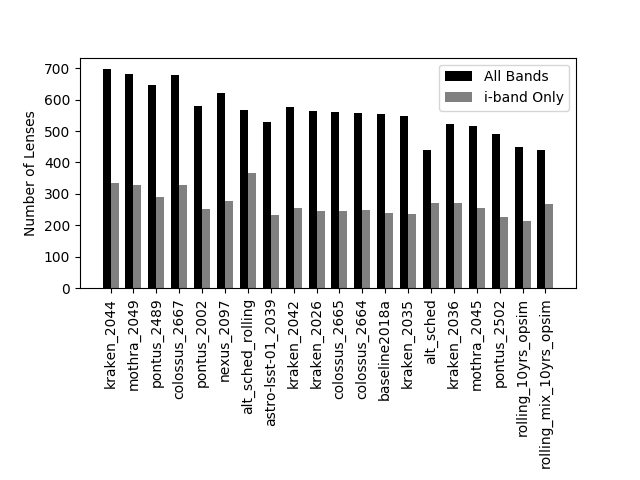
\includegraphics[width=\linewidth]{figures/sl_QSO_Nlens.png}    
		\caption{Number of ``golden lenses'' in sky areas with accuracies $<$0.2\%}   
\end{figure}

\begin{figure}
\centering
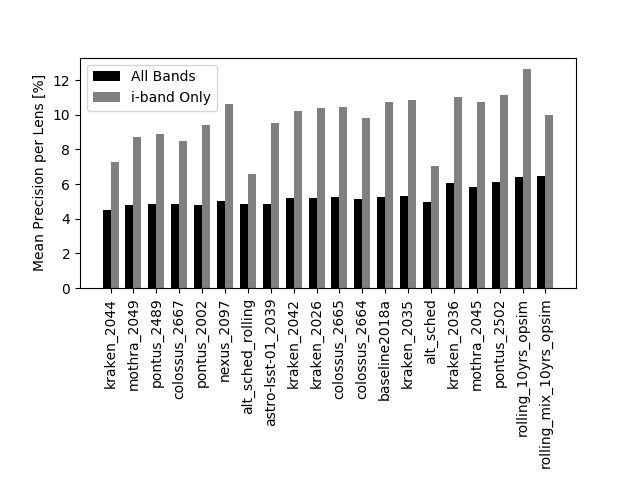
\includegraphics[width=\linewidth]{sl_QSO_Precision.png}    
		\caption{Mean precision per lens (percent) in  sky areas with accuracies $<$0.2\%}  
\end{figure}
\begin{figure}
\centering
		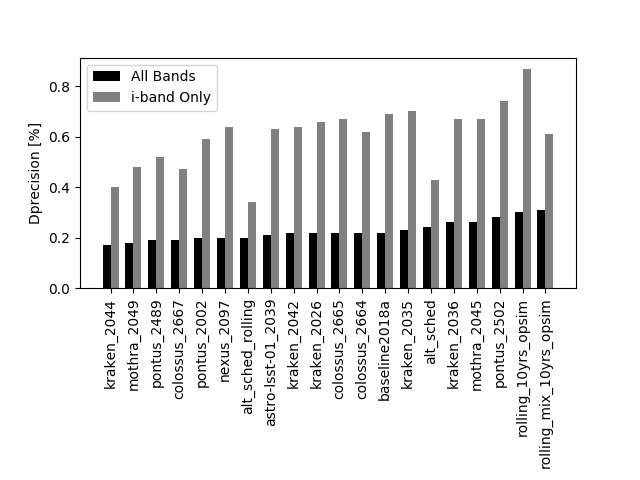
\includegraphics[width=\linewidth]{sl_QSO_Dprec.png}    
		\caption{Time delay distance precision figure of merit (percent) in  sky areas with accuracies $<$0.2\%} 
\end{figure}


\section{Supernovae}
\section{Weak Lensing}\label{sec:wl}

The LSST provides an opportunity to mitigate WL systematics using the observing strategy. This opportunity was not possible in previous surveys because the LSST will be the first survey to dither at large scales (relative to the field of view) with a large number of exposures.

We analyzed how different OpSim runs perform with respect to the point-spread function (PSF) modeling errors and similar WL systematics as follows: (a) We create 50 million stars uniformly in the WFD areas of each survey, with cuts based on the coadded depth and dust extinction, consistently the LSS WG. (b) we model the PSF modeling errors at each star in each exposure as a 6\% radial error in the outer 20\% of field of view (and no error). We assume an average size error on the PSF model of . This model is realistically motivated by recent surveys (e.g. \cite{bosche2018}) (c) We average down the modeling errors across exposures via their second moments, where this operation is linear. You can read more about this process on GitHub \footnote{\url{https://github.com/hsnee/lsstpsf/blob/master/methodology.ipynb}} (d) Propagate the averaged errors into bias on the cosmic shear using the $\rho$-statistics formulation (\cite{rowe2010}; \cite{jarvis2016}). The code to recreate this analysis is available on GitHub \footnote{\url{https://github.com/hsnee/lsstpsf/blob/master/ModelErrorsNew.ipynb}}. 

Figure~\ref{fig:WLSystematicsRankings} shows the result of this analysis, propagated into bias on the cosmic shear signal. 

Table~\ref{table:WLSystematicsRankings} provides a ranking of the strategies. There are certain trends that can be seen from the table (or equivalently, from figure~\ref{fig:WLSystematicsRanking}): more visits in the main WFD survey are very useful for averaging down weak lensing systematics (whether achieved by smaller area, or shorter 20 second visits.) OpSim runs with more exposure to the galactic planes underperform. Runs with rolling cadence significantly underperform others, especially ones that have rolling cadence in all or most years. These are not surprising trends, since prioritizing uniformity in WFD over area increases and rolling strategies is what would essentially drive weak lensing systematics down. Table~\ref{table:WLSystematicsRankings} also shows the average number of exposures in $i$-band for 5000 objects randomly drawn from a uniform distribution throughout the areas covered by each of the OpSim runs, and shows a strong correlation between this number and the performance of the runs. Rolling cadence runs and wider area runs also appear to have significant number of average visits. We are also exploring additional explanations of why rolling cadence runs are consistently underperforming.


\begin{figure}[hb]
    \centering
    \caption{The bias on the cosmic shear signal as a function of angular separation for all recent OpSim runs, at years 1, 3, 6, and 10. This indicates their performance with respect to weak lensing systematics, with higher curves corresponding to higher bias/worse performance.}
    \label{fig:WLSystematicsRankings}
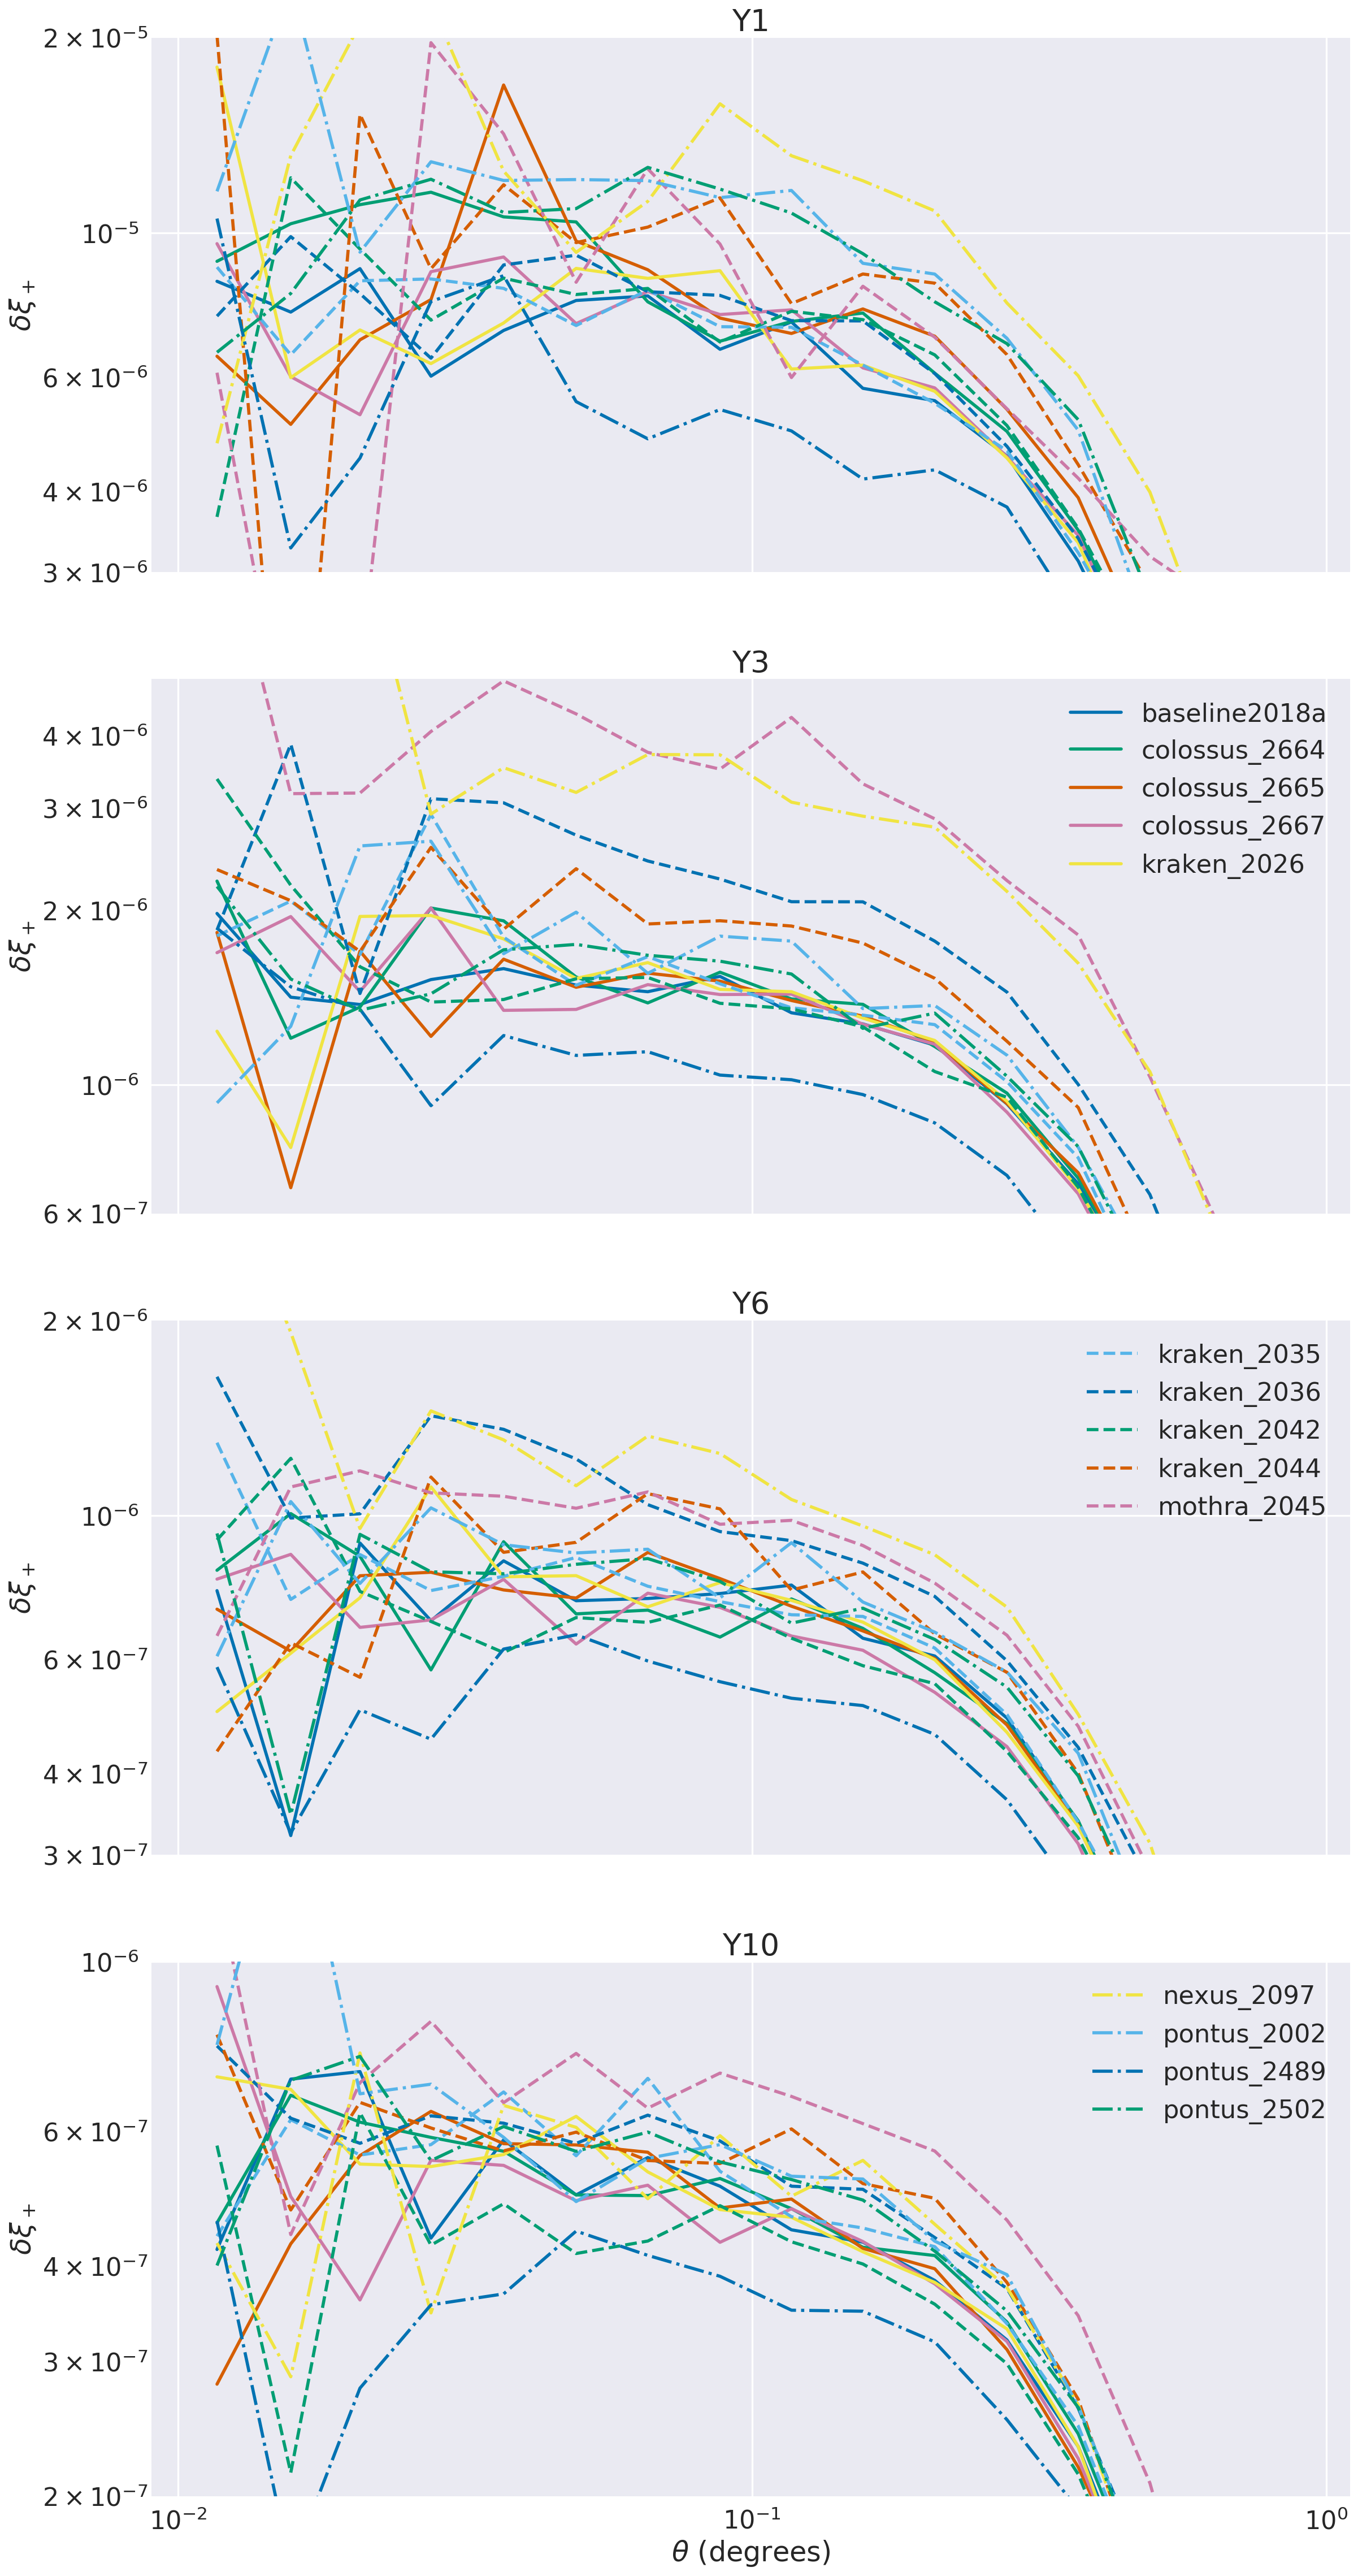
\includegraphics[width=0.72\textwidth]{figures/WLSystematicsAllYears.png}
\end{figure}




\begin{table}[ht]
\caption{A ranking of the recent observing strategies with respect to weak lensing systematics, as explained in the text, for years 1 and 10. Repeated numbers are ties. $<N>_i^{(Y10)}$ is the number of observations in $i$-band for objects on average after 10 years -- a simple metric that strongly correlates with the performance of an OpSim run, $<N>_i^{(Y10)}$ is typically higher for better-performing runs.}
\begin{tabular}{lllll}
\label{table:WLSystematicsRankings}
OpSim run & Y1 & Y10 & $<N>_i^{(Y10)}$ \\ \hline
mothra\_2045   & {\color{orange}9} & {\color{red}14}    & 134 \\
kraken\_2044   & {\color{red}11}   & {\color{red}13}    & 162 \\
nexus\_2097    & {\color{red}14}   & {\color{red}12}    & 159 \\
pontus\_2002   & {\color{red}12}   & {\color{red}11}    & 160 \\
kraken\_2036   & {\color{yellow}6} & {\color{orange}10} & 178 \\
pontus\_2502   & {\color{red} 12}  & {\color{orange}9}  & 179 \\
kraken\_2035   & {\color{green}2}  & {\color{yellow}8}  & 210 \\
colossus\_2664 & {\color{yellow}6} & {\color{yellow}7}  & 208 \\
kraken\_2026   & {\color{green}2}  & {\color{yellow}5}  & 217 \\
baseline2018a  & {\color{green}2}  & {\color{yellow}5}  & 212 \\
colossus\_2665 & {\color{orange}9} & {\color{green}3}   & 210 \\ 
colossus\_2667 & {\color{green}2}  & {\color{green}3}   & 220 \\
kraken\_2042   & {\color{orange}8} & {\color{green}2}   & 234 \\
pontus\_2489   & {\color{green}1}  & {\color{green}1}   & 306

\end{tabular}
\end{table}

There are several metrics that contain similar information to that in our analysis in MAF: the distribution of angles pointing to the center of the field of view in each observation \footnote{\url{https://github.com/LSST-nonproject/sims\_maf\_contrib/blob/5fd4ad762509cab0b4e403d84f2e65ed1ad08c06/science/static/WeakLensing\_Focal\_Angle.ipynb}} from Peter Yoachim which returns the Kolmogorov-Smirnov test's D-statistic for this distribution of angles against a uniform distribution, the distribution of coadded-depth (high values and narrow distribution is best) the distribution of airmass (low values and narrow distribution is best), the distribution of seeing values (also low values and narrow distribution is best). The reason these metrics provide similar results to our analysis is that survey uniformity is one of the crucial things that averages down WL systematics, and all these metrics are, in one way or another, a measure of uniformity.



\section{Static probes}

\newcommand{\todorm}[1]{\textbf{TO DO: #1}}

Here we present results for joint cosmological forecasts of the ``static'' probes: WL, LSS, and CL.
Unlike Section~\ref{sec:wl}, which focuses specifically on systematics mitigation for weak lensing,
this section focuses on dark energy constraining power.  The forecasting methodology follows
that in the DESC Science Requirements Document v1 \cite{DESCSRD2018}, though with modified
assumptions about the baseline LSST analysis for Y1 and Y10 based on the new strategies, and filling
in Y3 and Y6 forecasts as well. 
\todorm{Say more about the analysis, i.e., what is 3x2-point and how does CL fit in?}

We carried out forecasts for Y1, Y3, Y6, and Y10.  The reason for these choices is as follows: the
Y1 WL, CL, and LSS analysis will already be more powerful than all previous imaging surveys
combined, so first individual and joint-probe results will be produced at that time.  After that
point, there will likely be some regrouping to address whatever systematic uncertainties are
identified as the tallest poles in the Y1 analysis, so the next substantive analysis updates will
likely occur at Y3.  After this point Y6 and Y10 are somewhat arbitrary but suitably-spaced
benchmarks.  We use the Dark Energy Task Force (DETF \todorm{cite this!}) Figure of Merit
(FoM). \todorm{Define this if it hasn't been defined elsewhere in the writeup already.}

Given our adopted analyses, the following factors affect constraining power in the forecasts:
\begin{itemize}
\item Survey area $f_\text{sky}$: roughly speaking, with all other factors fixed, the FoM for WL,
  CL, and LSS scales like $f_\text{sky}^2$.  This assumes that noise terms that have a covariance
  that scales like $f_\text{sky}^{-1}$ dominate.  \todorm{Check scalings.}  A secondary impact of
  $f_\text{sky}$ is to modify the area overlap with spectroscopic surveys such as TiDES/4MOST and
  DESI, which will be used to place priors on photometric redshift biases and scatters
  \todorm{citations!}. The size of those priors therefore depends on $f_\text{sky}$ in some complex
  way related to the modifications in overlap with those two surveys.  However, this is a higher
  order effect that we will neglect in our initial analysis.
\item Survey median depth: Survey homogeneity is an important factor in precision measurements of
  galaxy densities, shears, and photometric redshifts.  We define a survey area after some depth
  cuts that are intended to roughly homogenize the area and eliminate regions with significant
  uncertainties due to dust reddening within the Milky Way.  These cuts are somewhat arbitrarily
  defined and could in principle be tuned for different strategies to maximize constraining power
  given the combination of depth and area factors.  The median survey depths after this cut, and
  their standard deviation, was discussed in the LSS section.  \todorm{Once Humna's text is visible,
    make this connection more clear/direct.}  The impact of the median survey depth is as follows:
  \begin{itemize}
    \item To modify the LSS tracer sample number density, assuming that we allow it to float in some
      way that is tied to the median depth.  The redshift distribution may also change.
    \item To modify the WL source sample number density; this sample is generally defined using a
      SNR cut rather than a strict magnitude cut.  The redshift distribution may also change.
    \item As shown in \cite{DESCSRD2018}, even going from Y1 to Y10, the number density changes are
      substantial while the redshift distribution changes are relatively modest.  Hence within a
      given year (e.g., all Y1 forecasts in this paper when considering all the strategies) we will
      focus on the changes in number density and neglect the differences in LSS and WL sample number
      redshift distribution between the strategies.  This simplifies the forecasting process.
  \end{itemize}
\item Photometric redshift quantity: this is tabulated in \todorm{refer to static tables or photo-z
  section once Humna and Melissa's work is included in the writeup}.  For a given size of prior on
  photo-z scatter and bias, modest changes (10s of percent) in photo-z quality do not have a
  significant impact on the forecasts, so we neglect this in the initial forecasts.
\end{itemize}

The above considerations have informed our approach to forecasting.  In particular, we group the
strategies based on those with similar usable areas and depths after the depth cuts described
above.  We only carry out forecasts for those groups of strategies, defined as follows
(\todorm{Consider turning this into a table, with FoM results and some explanation.}):
\begin{enumerate}
\item Y1: There are four groups of strategies: (1a) `mothra\_2045', (1b) `pontus\_2002', (1c)
  `pontus\_2502', and (1d) everything else.  The DESC SRD Y1 baseline had a median depth of 25.13 in
  $i$-band and an area of 12.3k~deg$^2$.  Group (1d) is quite similar to this in median depth and
  hence in number densities and redshift distributions, but with an area that is 14\% higher.  Group
  (1a) gives an increased depth by 0.4 magnitudes, which will substantially increase the WL and LSS
  number counts and modify their redshift distribution, but has a usable area 45\% below group (1d).
  Group (1b) is 0.2 magnitudes shallower than the DESC SRD Y1 baseline, but has the largest area,
  15.5k~deg$^2$; hence we have to make the LSS and WL sample number densities 20\% and 30\% lower
  than in the DESC SRD Y1 baseline, while keeping the redshift distribution fixed and accounting for
  the larger area.   Group (1c) has a similar depth as (1d) but 15\% smaller area than (1d), so can
  use the same forecasting parameters except for the area.
\item Y3: \todorm{}
\item Y6: \todorm{}
\item Y10: There are three groups of strategies: (10a) `mothra\_2045', (10b) `pontus\_2002' (largest
  area at 19.2k~deg$^2$, but shallowest and hence somewhat worse in terms of photo-z quality), and (10c)
  everything else (typically falling within $\pm 500$~deg$^2$ of 14.5k~deg$^2$).  The DESC SRD Y10
  baseline had a median depth of 26.35 in $i$-band and 14.3k~deg$^2$.  This is similar area to
  (10c), but roughly 0.2 mag shallower in median depth.  Roughly speaking, as mentioned above, we
  expect a modest change in the redshift distribution and no change in area for (10c) compared to
  the DESC SRD Y10 baseline, but the number density could increase by $\sim$20\% for LSS and $30$\%
  for WL.  In contrast, (10a) and (10b) are more similar in depth to the DESC SRD baseline, and
  hence we use the same number densities and redshift distributions, but with 19\% lower and 35\%
  higher areas than the DESC SRD baseline, respectively.
\end{enumerate}

\todorm{Tie results to LSS, WL section results.  Boil it down to simple statements about the
  features of the strategy that matter, rather than about these particular strategies.
  Consider iterative survey depth definition
  depending on the strategy.  Impact of high airmass, unusual seeing distributions, etc.  Impact of
  changes in DESI, 4MOST overlap.  Better quantification of photo-z impact.  Consistency of
  systematics and photo-z calculations with area/depth calculations.  Fitting formula for
  FoM given area and median depth.  Scatter as a function of redshift in the forecasts?}


\section{Joint Analysis}

\bibliographystyle{unsrt}
\bibliography{refs}


\end{document}
